\documentclass[a4paper,12pt]{book}

\usepackage[left=2.25cm,right=2.25cm,top=2.5cm,bottom=2.5cm]{geometry}
\usepackage[sc]{mathpazo}
\linespread{1.5}
\usepackage[T1]{fontenc}
\usepackage[utf8]{inputenc}
\usepackage[spanish]{babel}
\decimalpoint
\usepackage{graphicx}
\usepackage{listings}
\usepackage{color}
\usepackage{colortbl}
% Scalable fonts (para lettrine)
\usepackage{type1ec} 
\usepackage{lettrine}
% Cabeceras y pies de página
\usepackage{fancyhdr}
% Vertabim
\usepackage{moreverb}
% Código 
\usepackage{listings}
% Identacion y separacion de parrafos
\usepackage{parskip}
% Posicion de figuras
\usepackage{float}
% Diagramas
\usepackage[all,pdf]{xy}
% Subfiguras
\usepackage{subcaption}
% Hyperref
\usepackage{hyperref}
\hypersetup{
	colorlinks,%
	citecolor=black,%
	filecolor=black,%
	linkcolor=black,%
	urlcolor=black,%
	pageanchor=false
}
% URL en bibliografía
\usepackage{url}
% Apéndices
\usepackage{appendix}
% Múltiples columnas
\usepackage{multicol}
% Captions en multicols
\usepackage{caption}
% Títulos de capítulos
\usepackage{titlesec}
\titleformat{\chapter}[display]
{\bfseries\Large} 
{\filleft\MakeUppercase{\chaptertitlename} \Huge\thechapter} {4ex}
{\titlerule
\vspace{2ex}%
\filright} [\vspace{2ex}%
\titlerule]
% Tablas largas
\usepackage{longtable}
% Columnas de más de una fila en las tablas
\usepackage{multirow}
\usepackage{epstopdf}
\usepackage{setspace}

\renewcommand{\tablename}{Tabla}
\newcommand{\HRule}{\rule{\linewidth}{0.5mm}}
\renewcommand{\chaptermark}[1]{\lhead[{\sc{\chaptername\ #1}}]{}}
\renewcommand{\sectionmark}[1]{\rhead[ ]{{\thesection.\ #1}}}


\begin{document}
\title{Supervisión visual de normas COVID}
\author{Juan José Morell Fernández}

\begin{titlepage}
 
\begin{center}
 
% Upper part of the page
\vfill


\includegraphics[height=0.5\textwidth]{imagenes/escudo}\\[2.5cm]
 
\textsc{\LARGE Universidad de Murcia}\\[0.5cm]
 
\textsc{\Large Trabajo Final de Grado}\\[0.5cm]
 
% Title
\HRule \\[0.4cm]
{ \huge \bfseries Supervisión visual de}\\[0.4cm]
{ \huge \bfseries normas COVID}\\[0.4cm]
\HRule \\[1.5cm]
 
% Author and supervisor
\begin{minipage}{0.4\textwidth}
\begin{flushleft} \large
\emph{Autor:}\\
Juan José \textsc{Morell Fernández}\\
juanjose.morellf@um.es
\end{flushleft}
\end{minipage}
\begin{minipage}{0.4\textwidth}
\begin{flushright} \large
\emph{Tutor:} \\
Alberto \textsc{Ruiz Garcia}\\
a.ruiz@um.es
\end{flushright}
\end{minipage}
 
\vfill
 
% Bottom of the page
{\large \today}
 
\end{center}
 
\end{titlepage}

\let\cleardoublepage\newpage

\clearpage{\pagestyle{empty}\cleardoublepage}

% Agradecimientos
%!TEX root = proyecto.tex


\pagestyle{empty}

\vspace*{\fill}
\thispagestyle{empty}
\begin{quotation}
	\em 
	\begin{flushright}
		Those who can imagine anything, can create the impossible.
	\end{flushright}
	
	\medskip
	\raggedleft
	by Alan Turing 
\end{quotation}
\vspace*{\fill}
\clearpage{\pagestyle{empty}\cleardoublepage}

\pagestyle{plain}
\setcounter{page}1
\setcounter{secnumdepth}{4}	%Profundidad de la numeracion del indice
\setcounter{tocdepth}{2}	%Profundidad del indice

\linespread{1}
\tableofcontents
\clearpage{\pagestyle{empty}\cleardoublepage}
\linespread{1.5}

\listoffigures
%\listoftables
\clearpage{\pagestyle{empty}\cleardoublepage}

\setlength{\parindent}{18pt}

% Resumen en castellano
%!TEX root = proyecto.tex

\chapter*{Resumen}
\addcontentsline{toc}{chapter}{Resumen}

En 2020 comenzó una gran pandemia, provocada por el coronavirus (COVID-19), que está marcando la historia de la humanidad, y por un tiempo, paralizó todo el funcionamiento de la misma. Tal es la importancia del COVID-19, que la Organización Mundial de la Salud (OMS) presentó medidas para evitar el contagio entre personas. Entre ellas se encuentra la norma del uso de mascarillas para reducir el riesgo de la exposición de la población al virus. 

Para supervisar el uso correcto de las mascarillas en imágenes de personas, se plantea el uso de técnicas de visión artificial y \textit{machine learning} para la implementación de prototipos capaces de llevar a cabo dicho control en tiempo real. Para ello, se centra el esfuerzo en el estudio de las siguientes técnicas: \textit{Haar-like features}, \textit{Facial Landmarks}, \textit{Mediapipe}, \textit{Transfer Learning}/\textit{Tensorflow}. 

La primera técnica, \textit{Haar-like feature}, proviene de una investigación dirigida por Paul Viola y Michael Jones en el año 2001, centrada en el reconocimiento facial en tiempo real mediante el uso de dichas características y un modelo de \textit{machine learning} llamado Adaboost. Una vez detectada la cara, para identificar el uso de la mascarilla se usa un modelo SVM (\textit{support vector machine}), capaz de realizar regresiones y clasificaciones sobre un conjunto de datos, mediante la detección facial del modelo anterior.

La siguiente técnica, \textit{Facial Landmarks}, se apoya en la anterior (\textit{features}) para poder predecir puntos de interés del rostro humano, como: ojos, nariz y boca. Esto se logra por medio de una técnica llamada HOG (\textit{histogram of gradient}), que se basa en el estudio de la dirección de un punto en la imagen utilizando derivadas, logrando obtener unos datos que posteriormente serán utilizados en la creación de un clasificador SVM, capaz de realizar una detección/predicción en tiempo real. La implementación usada para el prototipo de esta técnica fue desarrollada por \textit{Kazemi} y \textit{Sullivan} en 2014.

Por otro lado, el tercer prototipo se centra en el uso de una de las soluciones implementadas en \textit{Mediapipe}, framework de Python desarrollado por Google para la creación de aplicaciones de visión artificial de forma sencilla y potente, llamada \textit{FaceMesh}. Junto a ella, se ha hecho uso de un modelo pre-entrenado de \textit{Haar-like features} y se ha construido un prototipo capaz de realizar detecciones en tiempo real con gran precisión. La idea de esta técnica es detectar un rostro en la imagen de entrada, obtener la zona donde se encuentra la boca del rostro y aplicar el modelo pre-entrenado para detectar si se encuentra una boca o no.

En último lugar, se implementó un prototipo con la técnica de \textit{Transfer Learning} y Tensorflow, plataforma que ha permitido su desarrollo. La idea consiste en la creación de un modelo personalizado para la detección de mascarillas. Concretamente se realizan un total de tres detecciones: mascarilla, no mascarilla, mal uso de la mascarilla. Para ello, se partirá de un modelo de \textit{Deep Learning}, llamado \textit{SSD-MobileNetV2}, y mediante el uso de \textit{Transfer Learning} se logra crear dicho modelo personalizado. Esta técnica se caracteriza por reusar un modelo ya entrenado para un nuevo problema.

Para terminar, se ha realizado una comparación entre todos los prototipos anteriores para estudiar cual de ellos ofrece el mejor control de la norma presentada por la OMS. Como resultado, no existe un único prototipo capaz de destacar sobre el resto en todos los ámbitos. Cada una de las técnicas empleadas pueden solucionar el problema, destacando al primer prototipo (\textit{haar-like features}) capaz de detectar rostros con mascarilla más lejanos, el tercer prototipo (\textit{Mediapipe}) como el más veloz y el prototipo cuatro (\textit{Tensorflow}) como el más acertado sobre el dataset, con un porcentaje de acierto del 40.27\% para el conjunto de test y un 43.8\% para todo el dataset con un 100\% de detecciones en ambos casos.


\clearpage{\pagestyle{empty}\cleardoublepage}

% Resumen en inglés
%!TEX root = proyecto.tex

\chapter*{Extended abstract}
\addcontentsline{toc}{chapter}{Extended abstract}

\vspace{-1.1cm}
The COVID-19 pandemic, also known as the coronavirus pandemic, is an ongoing global pandemic of coronavirus 2019 (SARS-CoV-2) disease that affects all the human population. The World Health Organization (WHO) declared a Public Health Emergency of International Concern regarding COVID-19 on January 30, 2020, and later declared a pandemic on March 11, 2020. This is why the WHO plublished an interim guidance to provide a updated recommendation on mask use in health care and community settings, and during home care for COVID-19 cases \cite{covid19}. This document contains updated evidence and guidance on mask management, virus (SARS-CoV-2) transmission, mask use by the public in areas with community and cluster transmission, mask use during vigorous intensity physical activity, etc. In addition, the WHO advises the use of masks as part of a comprehensive package of prevention and control measures to limit the spread of COVID-19 \cite{oms}. For this reason, this work will propose the use of Computer Vision and Machine Learning techniques for the implementation of prototypes capable of carrying out the visual supervision of correct mask use in real time. The effort will be focused on the study of the following techniques: Haar-like features, Facial Landmarks, Mediapipe, Transfer Learning / Tensorflow.

The first technique, Haar-like features, comes from an investigation directed by Paul Viola and Michael Jones in 2001, focused on real-time facial recognition using these type of features and a Machine Learning model called Adaboost. Moreover, paper \cite{paulViola} describes a machine learning approach for visual object detection which is capable of processing images fast and quite accurately. This research can be divided into three key concepts. The first is a new image representation called \textit{Integral Image}, which allows the features used to be computed faster during the execution of the algorithm. The second is a learning algorithm, based on AdaBoost, which selects a small set of features from a larger set of features and produces efficient classifiers. The third one is a method for combining those classifiers into a cascade architecture, which allows discarding background regions of the input image and spending more computation on promising object-like regions. Therefore, in real-time applications, a detector which use this technique is typicall able to run at 15 frames per seconds.

The first prototype is created by using an SVM (Support Vector Machine) model and an OpenCV face detector based on Haar-like features. This is a supervised learning model with associated learning algorithms that analyze data for classification and regresion analysis, and it is created by detections of the OpenCV's face detector itself, with images of faces with a mask and without it, obtaining a prototype that performs a detection that runs at 15 ms in real time with a good accuracy.

The second technique, Facial Landmarks, is implemented in the Dlib library for Python. It allows the recognition of points of interest on the faces that have been detected in the input image. The process that makes Dlib for this technique can be divided into two main steps: detecting faces within the image, and obtaining those points of interest. This implementation is based on the research of Kazemi and Sullivan in 2014, with the paper \textit{One Millisecond Face Alignment with an Ensemble of Regression Trees} \cite{faceLandmark}. This technique is capable of recognizing the following points of interest in a face: mouth, eyebrows, eyes, nose and chin, thanks to the use of an ensemble of regression trees, that can be used to estimate these points (\textit{facial landmarks}) directly from a sparse subset of pixel intensities.

The first step is to find a face within the input image, using the HOG (Histogram of Oriented Gradients) method. It follows an idea similar to the Haar-like features method, since it is based on the detection of features. The theoretical idea behind HOG is to find the appearance and shape of an object by analyzing the intensity of local gradients, thanks to the fact that these gradients have a greater magnitude in the vicinity of edges or corners. While deploying, it splits the image into small regions, called cells, and a one-dimensional gradient histogram is calculated for each of the pixels in each cell. The second step is to estimate the points of interest accurately and efficiently on the face. It is based on gradient boosting for learning an ensemble of regression trees, in charge of predicting the points of interest. 

Using OpenCV and the Dlib ToolKit, both ideas are implemented using pre-trained models. For facial detection and prediction of points of interest, it will be implemented with the models proposed by Dlib, more specifically the detection based on HOG and the prediction called \textit{shape\_predictor\_68\_face\_landmarks.dat}. The prototype created performs detections at 14.7 ms but with poor accuracy for this task. 

The third prototype is built with the use of Mediapipe, an API created by Google that offers customizable machine learning solutions for live and streaming media.
Google recommends Mediapipe to build prototypes by combining existing perception components, to advance them to polished cross-platform applications, and measure system perfomance and resource consumption on target platforms \cite{mediapipe}. Among the solutions it presents, there is a technique called Face Mesh that estimates 468 points of interest of a face, forming a 3D mesh in real time.

MediaPipe Face Mesh employs machine learning (ML) to infer the 3D surface geometry, requiring only a simple webcam like camera input. Using lightweight model architectures together with GPU acceleration throughout the pipeline, the solution delivers real-time performance critical for live experiences.

The pipeline used in this API consists of two Deep Learning models working at the same time. Its purpose is to perform a detection from an image of the points of interest on a face, and build a 3D face landmark model that approximates its surface by regression on said points. This task is facilitated if the face, where the points of interest must be detected, is clipped, thus making the model focus only on finding the points, increasing the precision of the prediction. Likewise, the cutouts of the faces can be generated from the previous predictions made by the same model, and the prediction is only called again when the presence of the face cannot be detected \cite{faceMesh}. All this is implemented thanks to the \textit{MediaPipe framework}. A pipeline is defined as a directed graph of components where each component is called a Calculator. These calculators are connected by data Streams. Each one represents a time-series of data Packets. So, the calculators and streams define a data-flow graph \cite{mediapipe}.

The prototype has been developed using FaceMesh from the MediaPipe API and a detector based on Haar-like features, such as the one mentioned in the Viola and Jones paper. Therefore, the idea behind this prototype is to obtain the area of the mouth thanks to the use of the solution provided by Mediapipe, and detect if there is a mouth in that area using a Haar-like features model implemented in OpenCV with a pre-trained model. The prototype makes detections at 12.3 ms with good precision and accuracy at short distances. 

The last prototype uses the Transfer Learning technique, and for that reason the use of Tensorflow is necessary. It is an Open Source platform dedicated to machine learning, that allows us to easily compile and deploy ML technology applications. It is based on tensors, multidimensional arrays with a uniform type, like np.arrays in Numpy. In the field of computer vision, it has a large number of pre-trained models capable of performing object detection and image classification quickly and accurately. This resource is called TensorFlow Model Garden, and it is a repository with different model implementations and solutions modeled for Tensorflow. The models are pre-trained using a dataset called COCO 2017. This is a large data set on a large scale for object detection, segmentation, and capture. Among these models, MobileNet stands out, capable of obtaining great performance on mobile devices and computers with little computational power. This has created a rise in popularity for detector implementations on embedded devices, such as the Raspberry Pi, or on ESP32 chips using remote processing.

The goal of this prototype is to use Transfer Learning on the MobileNet model to retrain it for our task. Transfer Learning is a technique in which a pre-trained model is reused for a new problem. Currently its use is becoming popular, since it allows the training of a deep neural network with a small amount of data. In this case, the aim is to use a general object detection model and, applying transfer learning, re-train it for a more specific task but without wasting its previous knowledge. 

The prototype has been built with the use of an SSD-MobileNet model, a combination of an SSD (Single Shot MultiBox Detector) model with another model called MobileNet. This type of model is characterized by the use of a method to detect objects in images using a deep neural network, which generates prediction values about the presence of each object / category in each of the detections, and returns the object with the highest match. The dataset used in Transfer Learning is a combination of datasets composed of images of people with a mask, without it and with the mask incorrectly placed. It consists of a total of 895 images, divided into two groups: train and test. The first group contains the images that are used to train the model and has 745 images. Whereas, the test set is used to validate the trained model, and it has 150 images. Once the images are selected, the labeling process is carried out, using a program created with Python called labelImg. 

To perform Transfer Learning using Tensorflow, the following configuration files need to be created: \textit{LabelMap}, two \textit{TFRecord} files, and \textit{pipeline.config}. This last file contains the main information of the model, both the number of classes that it can detect, the size that the images are resized before treating them, and checkpoints for training. For its creation, the use of Protobuf will be necessary. This is a Google tool focused on transforming the xml files generated by labeling the images in protocol buffers, to serialize the information in a structured and faster way. To carry out the training, we use the code provided after the installation of the Tensorflow Object Detection API, called \textit{model\_main\_tf2}. After training, files called checkpoints are obtained, which contains the model that can be loaded for use in Tensorflow. Once the prototype is created, detections are made in a time of 83.3 ms, making the detections slower than the rest of the prototypes created but being a more scalable project.

Tree metrics are used to compare the prototypes. The first comparison is based on the study of the working range of the prototypes, by measuring distance by the size of the detection that the algorithm implemented in the prototype can perform. The second comparison is based on the measure of the time the algorithm takes to process an input image. For this, the same test will be carried out on all prototypes, and the average time (ms) is calculated after an execution of one minute. Finally, the third comparison will study the percentage of correct classifications for the dataset built in this project. All the experiments have been executed in a PC with Intel i7 processor at 1.3GHz and 8 cores, Intel Iris Plus Graphics GPU, 8 Gb of RAM, and Ubuntu version 18.04.

As a result, there is no single prototype capable of standing out across the board, making it impossible to select an optimal solution to the problem in all cases. All the techniques used in this work can solve it and, depending on where the prototype will be applied, another study would have to be carried out to solve these specific objectives. For example, if we wanted to implement a detector of this type in a mobile device or in an embedded system, it would be preferable a prototype that is fast and light, such as the third prototype (Mediapipe). Whereas, if we have a device with more computing power, it could considered using a slower but more precise prototype such as the first one (Haar-like features) or even training a custom model such as the fourth prototype (Transfer Learning). Therefore, a preliminary study should be carried out on the device where the prototype will be applied to make a final decision.




\clearpage{\pagestyle{empty}\cleardoublepage}

\pagestyle{fancy}
\renewcommand{\chaptermark}[1]{\lhead[{\sc{\chaptername\ \thechapter.\ #1}}]{}}
\renewcommand{\sectionmark}[1]{\rhead[ ]{{\thesection.\ #1}}}
\renewcommand{\headrulewidth}{0.5pt}
\renewcommand{\footrulewidth}{0.5pt}

% Introduccion
%!TEX root = proyecto.tex

\chapter{Introducción}

\lettrine[lines=4]{L}{a} visión artificial  es un ámbito de la informática que surgió hace 60 años, pensado en el estudio del procesamiento digital de las imágenes. En los últimos años ha tomado mucha importancia el reconocimiento facial, algoritmo capaz de identificar rostros humanos dentro de una imagen,  gracias a la investigación realizada por \textit{Viola y Jones} en 2001, y la reciente tendencia en \textit{smartphones} con el desbloqueo facial. 

\section{Historia de la Visión Artificial}

Uno de los primeros acontecimientos que propició la visión artificial fue la creación del cable Bartlane, capaz de transmitir una imagen a través del mar atlántico en los años 1920, con una duración de cerca a una semana. Pero, dentro del entorno del procesamiento de imágenes digitales, la investigación se centró en recuperar una estructura tridimensional del mundo real a través de una imagen para conseguir un entendimiento total de la escena que plasma la misma. Debido a esto aparecieron varios algoritmos de reconocimiento de lineas, donde uno de ellos fue creado por parte de Huffman en 1971.

Pero el avance de estas investigaciones pronto se ligarían con el del ordenador. Estos, se podrían resumir en varios acontecimientos importantes, tales como: la invención del transistor por Bell Laboratories en 1948 y de los circuitos integrados en 1958 o la introducción por parte de IBM de los primeros ordenadores personales en 1981. \cite{gonzalez_woods_2018}

Uno de los descubrimientos que inicio este movimiento no fue proveniente de la informática, sino de la psicología. Esta sería una de las principales fuentes sobre el entendimiento de como funciona la visión.  Un par de psicólogos, David Hubel y Torsten Wiesel, describieron que el comportamiento de las neuronas encargadas de entender el entorno visual siempre empiezan con estructuras simples como vértices. Más tarde esta idea se convertirá en el principio central del \textit{Deep Learning}.

Russell Kirsch, en 1959, es el primero en desarrollar un aparato que traducía las imágenes en datos que las máquinas pudiesen entender. Y, Lawrence Roberts en 1963 publica un estudio sobre como las máquinas perciben objetos sólidos de tres dimensiones, uno de los avances considerados precursores de la visión artificial moderna.

Durante los años 1980s, se desarrolló una red artificial capaz de reconocer patrones, mediante el uso de una red convolucional. Que propició la creación de un modelo llamado LeNet-5, la primera red convolucional moderna. Este modelo se caracteriza por usar la backpropagación. Mientras que en los años 1990s la visión artificial cambia totalmente de rumbo y los investigadores pasaron de intentar reconstruir objetos en 3D a intentar detectar objetos mediante sus características.

A partir del año 2000 se hacen muchos avances importantes y que actualmente son usados en aplicaciones reales. El primer detector facial llegaría en 2001 creado por Paul Viola y Michael Jones. Ambos consiguieron crear el primero que funcionase en tiempo real.

El problema de estos modelos es el uso de información para poder entrenarlos, y para esto se creo un proyecto llamado PASCAL VOC, que creo un dataset estándar para la clasificación de objetos. Posteriormente, apareció en 2010 ImageNet, el cual contiene más de un millón de imágenes para un total de mil objetos. Y junto a este apareció un modelo basado en una red convolucional llamado AlexNet. Desde entonces, el \textit{Deep Learning} se ha convertido en eje central del avance en la visión artificial, conjuntamente con todos los avances matemáticos realizados anteriormente.

\section{Reconocimiento Facial y COVID-19}

En la actualidad, la visión artificial se utiliza en muchos proyectos y esta presente en investigaciones muy importantes para el futuro de la inteligencia artificial. Una de ellas se basa en el reconocimiento facial, y es usado en aplicaciones para reconocer personas, aspectos, contador de personas, etc. 

La detección facial se inicia con una imagen arbitraria, con el objetivo de encontrar todas las caras que hay en una imagen, y posteriormente devolver otra con la localización exacta de cada una de las caras. Aunque esta tarea es natural para los humanos, es bastante complicada para los ordenadores. Ya que se encuentran muchos factores que lo dificultan, tales como: la escala, localización, punto de vista, iluminación, lentes, etc. Existen centenares de investigación/proyectos de detección facial, desde uno de los mas influyentes en los años 2000s, como \textit{Viola and Jones face detection}, a proyectos basados en \textit{Deep Learning}, con tecnologías como \textit{Tensorflow} o \textit{YOLO}. \cite{szeliski_2018}

Tras el año 2020 y la aparición del COVID-19, el uso de mascarillas y el cumplimiento de las normas impuestas por la OMS (Organización Mundial de la Salud) están al orden del día. En este trabajo se tendrá como objetivo el estudio de todas estas tecnologías para poder controlar dichas normas, terminando con un prototipo capaz de detectar cuando una personas lleva mascarilla, ya sea al entrar a un comercio, evento u trabajo.




% Estado del arte
%!TEX root = proyecto.tex

\chapter{Estado del arte}

El reconocimiento facial es un ámbito de la visión artificial, que como su nombre indica, se centra en la búsqueda de rostros humanos dentro de imágenes digitales. Durante años se han desarrollado varias tecnologías capaces de realizar dicha acción, de las que se pueden distinguir dos grupos: aplicaciones con y sin el uso de \textit{Deep Learning}. Aunque, ambos se centran en las características de los rostros humanos para lograr identificarlos. Conocidas como \textit{features}, que corresponden con puntos de la cara muy reconocibles, como: el mentón, ojos, cejas, nariz, etc. Esta técnica fue usada por primera vez en 2001, por Paul Viola y Michael Jones, y desde entonces se ha convertido en unas de las técnicas principales en el reconocimiento facial.

Este ejercicio se complica cuando las imágenes presentan errores naturales en su toma (como baja luz, ruido, etc.) o los individuos visten complementos que tapen sus rasgos faciales. Este es el problema que se va a plantear en este trabajo, buscar una posible solución al reconocimiento facial con complementos faciales, en especifico identificar si las personas llevan mascarillas.

\section{Python y OpenCV}

Python es un lenguaje de programación \textit{Open Source} y de alto nivel, que permite trabajar y desarrollar aplicaciones de forma rápida y sencilla. Además, se trata de un lenguaje que ha aumentado en popularidad los últimos años gracias a su gran uso en ramas de la tecnología emergente, como \textit{Data Science}, Inteligencia Artificial, \textit{Big Data} o Visión Artificial. En esta última gracias a la existencia de una herramienta llamada \textit{OpenCV}, librería \textit{Open Source} centrada en la creación de aplicaciones en tiempo real sobre visión artificial, que cuenta con una gran cantidad de implementaciones de algoritmos de \textit{Computer Vision}.

\section{Aplicaciones sin Deep Learning}

Entre los años 2000 y 2015 se implementaron varias soluciones para el problema de la identificación facial. Centrados, su mayoría, en la extracción de caracteristicas del rostro humano mediante técnicas de procesamiento de imágenes digitales. Son importante de destacar los siguientes avances durante estos años:

\begin{enumerate}
	\item \textbf{HAAR-like Features \& ADABOOST}.
	
	Técnica diseñada por Paul Viola y Michael Jones en el año 2001, donde se implementa una detección mediante el uso de \textit{Machine Learning} que es capaz de procesar imágenes a una velocidad y precisión bastante altos, comparado con los desarrollos de la época, gracias al uso de técnicas avanzadas de procesamiento de imágenes y de un modelo de \textit{Machine Learning} llamado \textit{AdaBoost} \cite{paulViola}. 
	
	\item \textbf{HOG} (Histogram of Gradient).
	
	Se trata de una técnica de detección de rostros u otro tipo de objetos mediante el uso de gradientes, término dedicado al estudio de la dirección de un punto en la imagen utilizando derivadas. Estos servirán para el entrenamiento de un clasificador SVM (\textit{Super Vector Machine}), que será capaz de realizar una detección en tiempo real.
	
	\item \textbf{Facial Landmarks}.
	
	Con la aparición de técnicas como las anteriores, se dio el siguiente paso con la predicción de puntos de interés sobre los rostros detectados. El desarrollo de esta se realiza con el uso de técnicas llamadas: \textit{Gradient Boosting} y \textit{Ensemble of regression trees}, ambas del ámbito del \textit{Machine Learning} \cite{faceLandmark}. Cabe destacar, que esta técnica detecta rasgos faciales (como boca, nariz u ojos) aunque se encuentren escondidos tras algún complemento u objeto, gracias al uso de la predicción.
\end{enumerate}


\section{Aplicaciones con Deep Learning}

A partir de 2016, el \textit{Deep Learning} fue un ámbito que gano mucha importancia en la visión artificial. Basado en estructuras CNN (\textit{Convolutional Neural Network}), capaces de extraer las características de las imágenes de entrada mediante el uso de filtros. Algunas de las principales implementaciones del \textit{Deep Learning} para la detección de objetos/rostros son:

\begin{enumerate}
	\item \textbf{YOLO}.
	
	Modelo capaz de procesar imágenes en tiempo real a una velocidad de 45 frames por segundo (con una GPU Nvidia Titan X), con el uso de una única red convolucional (CNN) que predice simultáneamente varios tipos de clases de objetos. Este modelo es entrenado mediante imágenes completas \cite{YOLO}.
	
	\item \textbf{TensorFlow}.
	
	TensorFlow es una plataforma de \textit{Open Source} dedicada al aprendizaje automático. Permite compilar e implementar con facilidad aplicaciones con tecnología de AA. En el ámbito de la visión artificial, dispone de una gran cantidad de modelos pre-entrenados capaces de realizar detección de objetos y clasificación de imágenes de forma rápida y precisa. Entre dichos modelos destaca \textit{MobileNet}, capaz de obtener un gran rendimiento en dispositivos móviles y ordenadores con poca potencia computacional. Esto ha creado un aumento de la popularidad en la implementaciones de detectores en dispositivos embebidos, como \textit{Raspberry Pi}, o en chips ESP32 mediante procesamiento remoto.
	
	\item \textbf{MediaPipe}.
	
	MediaPipe \cite{mediapipe} es un framework creado por Google centrado en el desarrollo de aplicaciones de visión artificial de forma sencilla y potente. Este se basa en un modelo propio llamado BlazeFace, inspirado en modelos como MobileNet. Entre sus soluciones (Figura \ref{fig:solMed}) se pueden encontrar: detección facial, predicción de una malla facial (Face Landmarks), detector de iris, detector de manos, reconocer poses, segmentación de pelo, etc.
	
	\begin{figure}[htp]
		\centering
		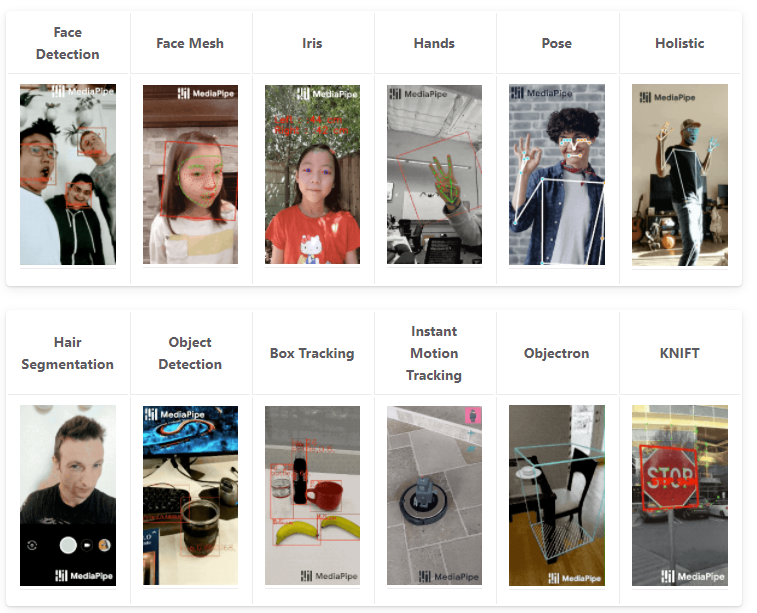
\includegraphics[width=10cm]{imagenes/solucionesMediaPipe.png}
		\caption{Soluciones de MediaPipe \cite{mdSolutions}.}
		\label{fig:solMed}
	\end{figure}
	
	\item \textbf{IBM Watson}.
	
	IBM Watson es un servicio ofrecido por IBM, que permite la creación de aplicaciones de inteligencia artificial en la nube. Este tipo de servicios nos permiten crear aplicaciones potentes sin necesidad de disponer de una gran potencia computacional en nuestra casa. Concretamente, IBM Watson dispone de un modulo llamado \textit{Visual Recognition} que permite el análisis de imágenes y detección de objetos. Este tipo de servicios son de pago, pero permiten una cantidad de procesado gratuita. En este caso, IBM permite tener dos modelos personalizados y 1000 eventos de forma gratuita al mes \cite{ibm}. 
\end{enumerate}





% Análisis de objetivos y metodología 
%!TEX root = proyecto.tex

\lstset{frame=single,basicstyle=\ttfamily\small}

\chapter{Análisis de objetivos y metodología}
\vspace{-1cm}
El COVID-19 es un virus que ha provocado en la humanidad incontables problemas, y en el mundo de la visión artificial también, por eso me voy a centrar en la creación de un prototipo que sea capaz de revisar el cumplimiento de las normas COVID impuestas en España y en todo el mundo por la OMS. Concretamente, detectar cuando una persona lleva, de manera correcta, una mascarilla al entrar a un comercio, cine, restaurante, etc. Los objetivos que se plantean para llevar esto a cabo son los siguientes:

\begin{itemize}
	\item Estudio de las tecnologías actuales, para comprobar su comportamiento con uso de mascarilla.
	\item Creación de un prototipo capaz de reconocer rostros y detectar si se lleva mascarilla.
	\item Estudiar la capacidad de que el prototipo pueda identificar si se lleva correctamente la mascarilla. 
	\item Poder detectar la mascarilla, independientemente del tipo que se lleve.
\end{itemize}
\vspace{-0.7cm}
\section{Prototipo}
\vspace{-0.5cm}
Para cada uno de los apartados del desarrollo de este \textit{TFG} se creará un prototipo con la finalidad de mostrar la tecnología expuesta en el mismo, con el objetivo final de crear una aplicación que contenga todos los prototipos y se puedan ejecutar de forma sencilla. 

Los prototipos serán probados en varios escenarios de prueba, todos ellos se realizarán en tiempo real. Se contará con una totalidad de tres escenarios:

\begin{itemize}
	\item Detección de mascarillas a una distancia cercana.
	\item Detección de mascarillas a una distancia media.
	\item Detección de mascarillas desde una posición alejada.
\end{itemize}

Asimismo, las pruebas se repetirán en dos dispositivos diferentes. El primero de ellos sin GPU y el segundo con GPU (CUDA). A continuación se muestran las especificaciones de los dispositivos:

\begin{table}[h!]
	\begin{center}
		\begin{tabular}{ |c|c|c|c| } 
			\hline
			 & PC 1 & PC 2 \\
			\hline
			\multirow{3}{4em}{CPU} & Intel i7-1065G7 & Intel i7-6700HQ \\ 
			& 1.30GHz & 2.60GHz \\ 
			& 8 núcleos & 8 núcleos \\ 
			\hline
			GPU & Intel Iris Plus Graphics  & GTX 980M 2Gb \\
			\hline
			CUDA & NO  & SI \\
			\hline
			RAM & 16 Gb & 8 Gb \\
			\hline
			OS & Ubuntu 18.04 & Ubuntu 18.04 \\
			\hline
		\end{tabular}
		\caption{Entornos de prueba.}
		\label{tab:table1}
	\end{center}
\end{table}

Por último, serán probados bajo un mismo \textit{dataset} (mostrado en el apartado \ref{dataset}) para calcular el porcentaje de aciertos y detecciones que consiguen cada uno de ellos.

\vspace{-0.9cm}
\section*{Herramientas}
\vspace{-0.5cm}

Para el desarrollo del prototipo se hará uso del lenguaje de programación de alto nivel, Python. Junto a este se usarán las siguientes herramientas:

\begin{itemize}
	\item \textit{OpenCV}: Librería \textit{Open Source} centrada en la creación de aplicaciones en tiempo real sobre visión artificial, que cuenta con una gran cantidad de implementaciones de algoritmos de visión artificial.
	\item \textit{Dlib}: Librería compuesta por implementaciones de algoritmos \textit{Machine Learning}, centrada en la creación de aplicaciones que resuelven problemas del mundo real. En concreto se hará uso de su apartado de \textit{HOG detector} y \textit{Facial Landmark}.
	\item \textit{Scikit-learn}: Librería de \textit{Machine Learning} capaz de realizar clasificación, regresión, \textit{support vector machine} (SVM), \textit{gradient boosting, \textit{k-mean}}, etc. Se implementa conjuntamente con las librerías Numpy y SciPy.
	\item \textit{Numpy}: Librería que añade funcionalidad a \textit{arrays} multidimensionales y matrices, junto a un gran conjunto de operaciones matemáticas para trabajar con ellos.
	\item \textit{Mediapipe}: Librería con soluciones y aplicaciones de \textit{Machine Learning} para dispositivos móviles, en la nube o web.
	\item \textit{Tensorflow}: Librería de \textit{Machine Learning}, referente a el entrenamiento y utilización de redes convolucionales (\textit{Deep Learning}).
\end{itemize}

\vspace{-1cm}
\section*{Fases de desarrollo}
\vspace{-0.5cm}
El proceso de implementación del prototipo en cada una de las técnicas presentadas en este TFG, van a contar con el siguiente flujo de trabajo:

\begin{enumerate}
	\item \textit{Investigación}: El primer paso, se centra en la investigación del funcionamiento de la técnica a estudiar. Priorizando el estudio del \textit{paper}, artículo oficial donde se presenta la técnica por sus autores. Y, posteriormente buscar información extra en libros u artículos web.
	\item \textit{Implementación básica}: EL segundo paso se trata de realizar una implementación de la técnica estudiada, tal y como se presenta por los autores. Con el objetivo de realizar un estudio de precisión y rapidez.
	\item \textit{Implementación propia}: Por último, se crea un prototipo de la técnica intentando resolver los objetivos establecidos. Recabando datos, para una comparación final entre todas las técnicas estudiadas.
\end{enumerate}

\vspace{-0.7cm}
\section*{Dataset} \label{dataset}
\vspace{-0.5cm}

Un \textit{dataset} es un conjunto de imágenes utilizado para realizar el entrenamiento y validación de un modelo de \textit{Machine Learning}. En este trabajo se hará uso de la combinación de dos \textit{dataset} existentes para representar todas las posibilidades del problema planteado, conteniendo imágenes de personas con mascarilla, sin ella y con ella pero mal colocada. El primer dataset de la combinación proviene de \textit{Kaggle} llamado \textit{Covid face mask detection dataset} \cite{datasetMask} (Figura \ref{fig:1}). Kaggle es una comunidad de \textit{Machine Learning} y \textit{Deep Learning} donde se comparten proyectos y dataset. Mientras que, el segundo dataset proviene de una investigación \cite{Cabani_2021}, llamada \textit{Maskedface-net}, centrada en la creación de imágenes de personas donde se muestre un mal uso de la mascarilla (Figura \ref{fig:1}). Finalmente, el dataset creado para este trabajo cuenta con un total de 895 imágenes, donde 745 formarán el conjunto de entrenamiento y 150 el de test.

\vspace{0.3cm}

\begin{figure}[htp]
	\centering
	\begin{subfigure}{0.2\linewidth}
		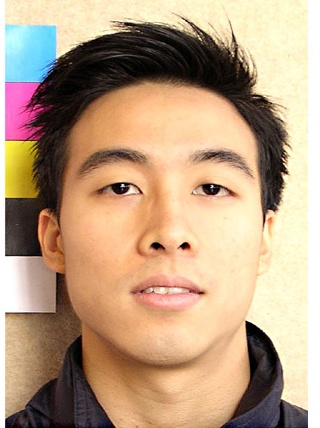
\includegraphics[width=\linewidth]{imagenes/dataset1-1.jpg} 
		\caption{}
		\label{fig:1a}
	\end{subfigure}\hfill
	\begin{subfigure}{0.2\linewidth}
		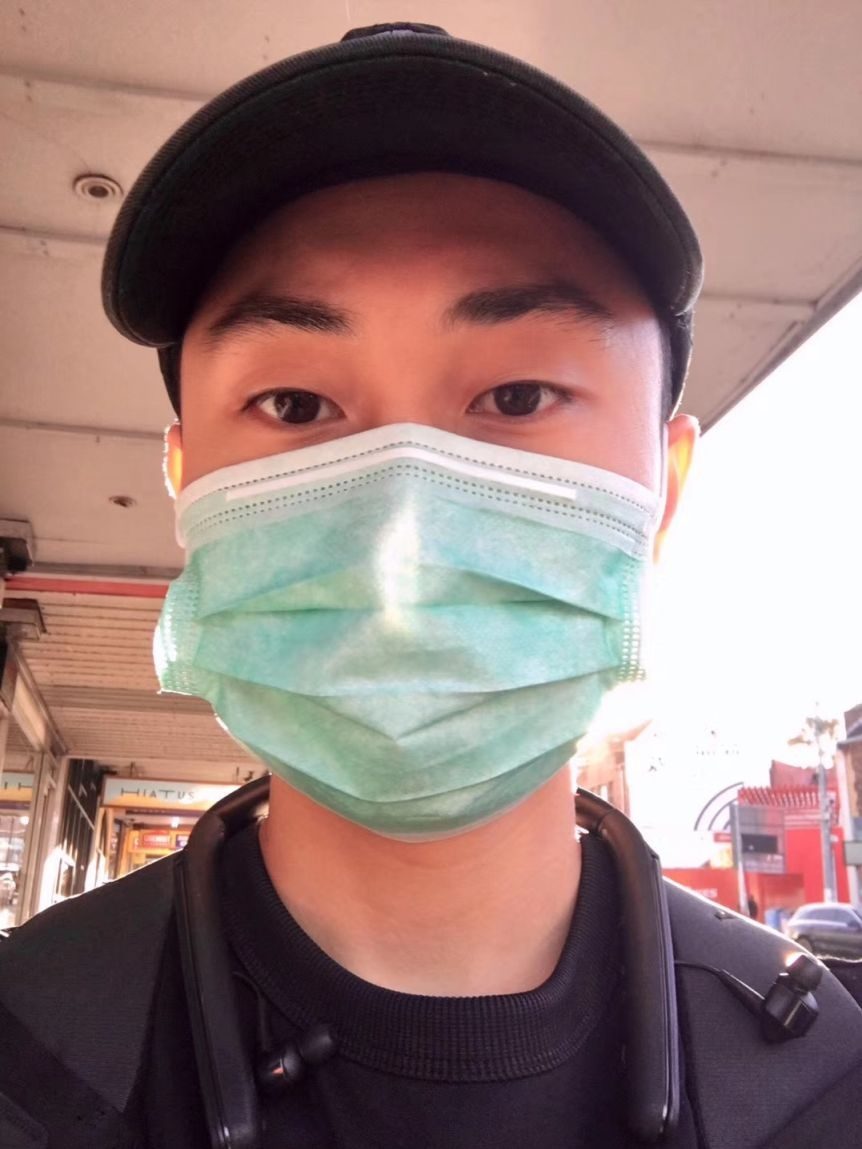
\includegraphics[width=\linewidth]{imagenes/dataset1-2.jpg}
		\caption{}
		\label{fig:1b}
	\end{subfigure}\hfill	
	\begin{subfigure}{0.2\linewidth}
		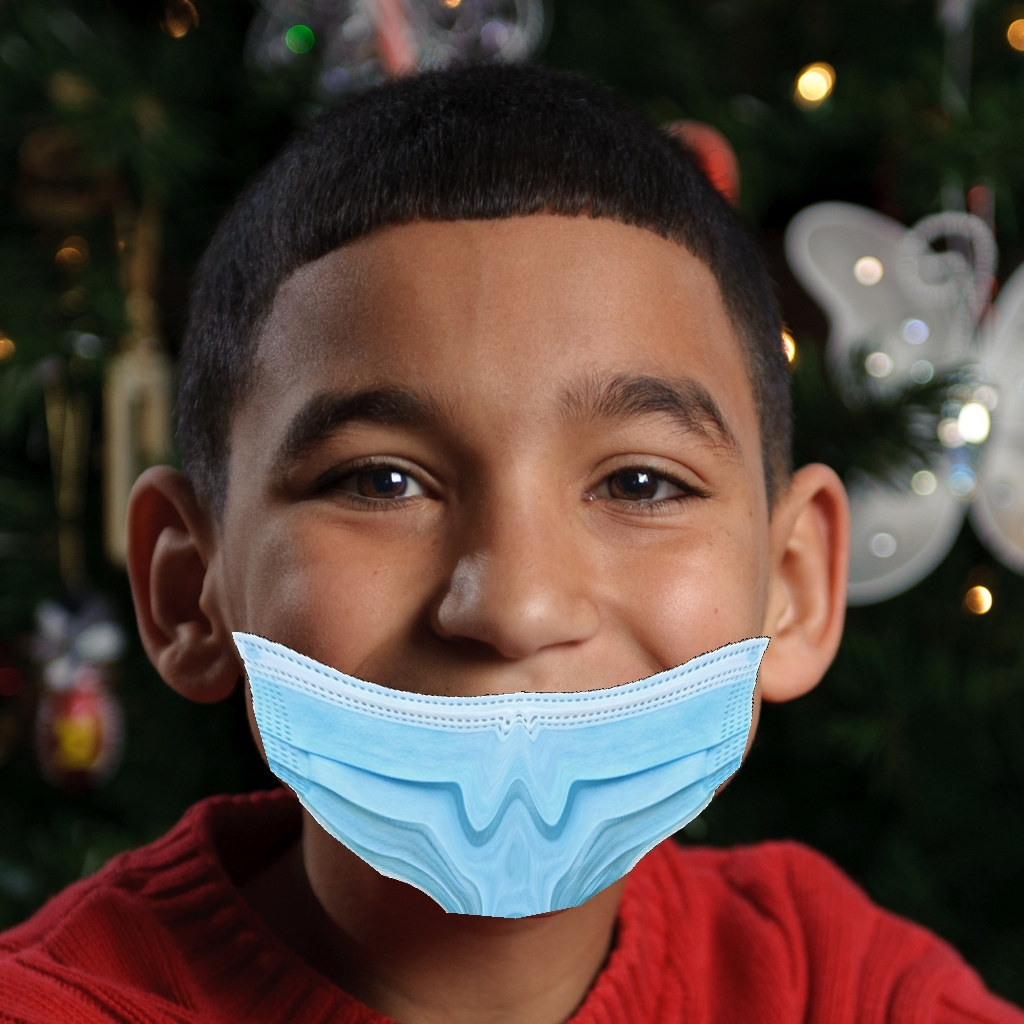
\includegraphics[width=\linewidth]{imagenes/dataset1-3.jpg}
		\caption{}
		\label{fig:1c}
	\end{subfigure}
	\newline
	\begin{subfigure}{0.2\linewidth}
		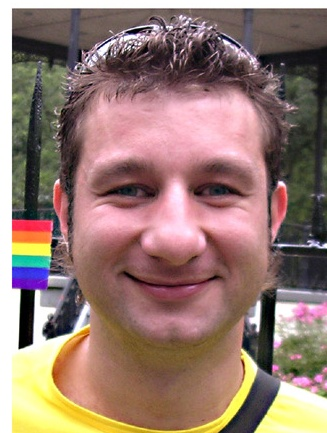
\includegraphics[width=\linewidth]{imagenes/dataset1-4.jpg} 
		\caption{}
		\label{fig:1d}
	\end{subfigure}\hfill
	\begin{subfigure}{0.2\linewidth}
		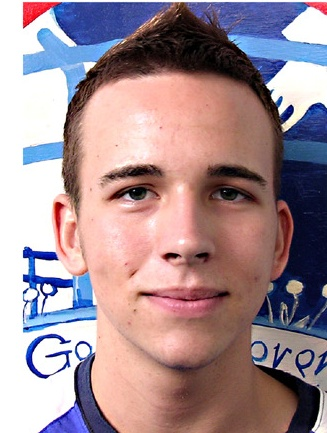
\includegraphics[width=\linewidth]{imagenes/dataset1-5.jpg}
		\caption{}
		\label{fig:1e}
	\end{subfigure}\hfill	
	\begin{subfigure}{0.2\linewidth}
		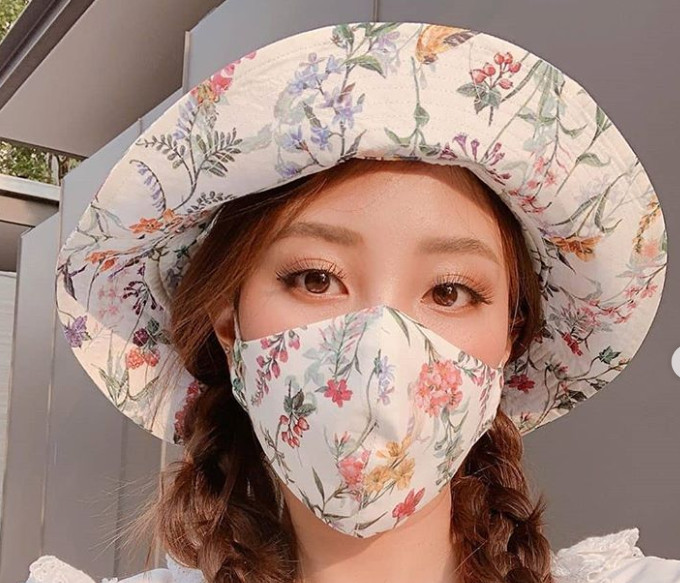
\includegraphics[width=\linewidth]{imagenes/dataset1-6.jpg}
		\caption{}
		\label{fig:1f}
	\end{subfigure}
	\newline
	\begin{subfigure}{0.2\linewidth}
		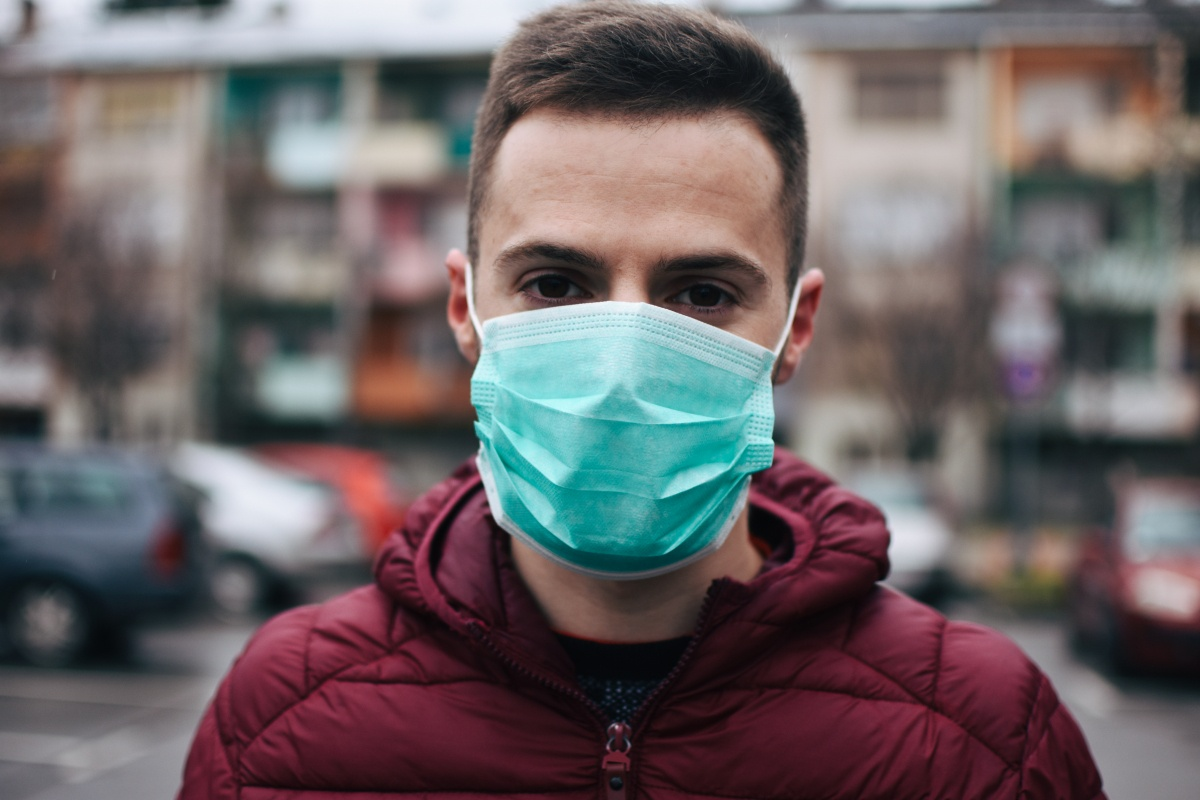
\includegraphics[width=\linewidth]{imagenes/dataset1-7.jpg} 
		\caption{}
		\label{fig:1g}
	\end{subfigure}\hfill
	\begin{subfigure}{0.2\linewidth}
		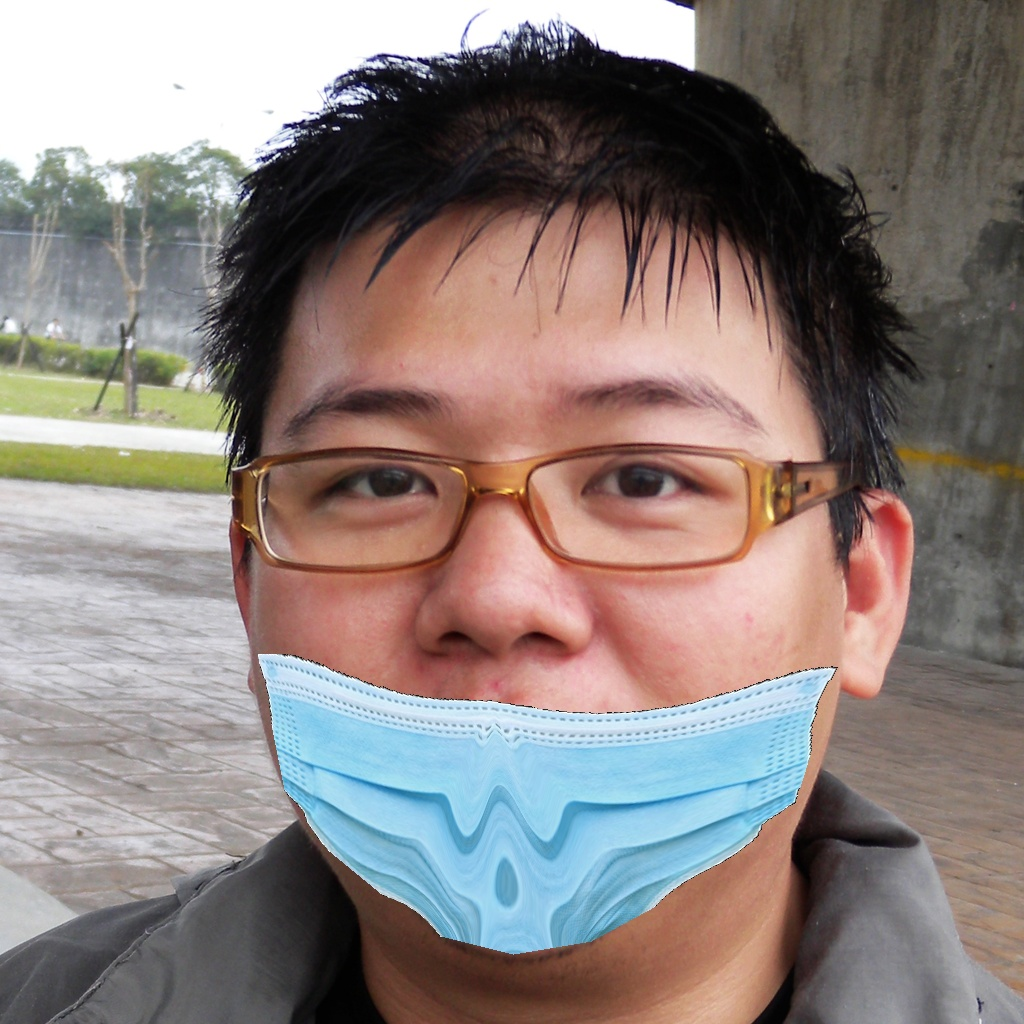
\includegraphics[width=\linewidth]{imagenes/dataset1-8.jpg}
		\caption{}
		\label{fig:1h}
	\end{subfigure}\hfill	
	\begin{subfigure}{0.2\linewidth}
		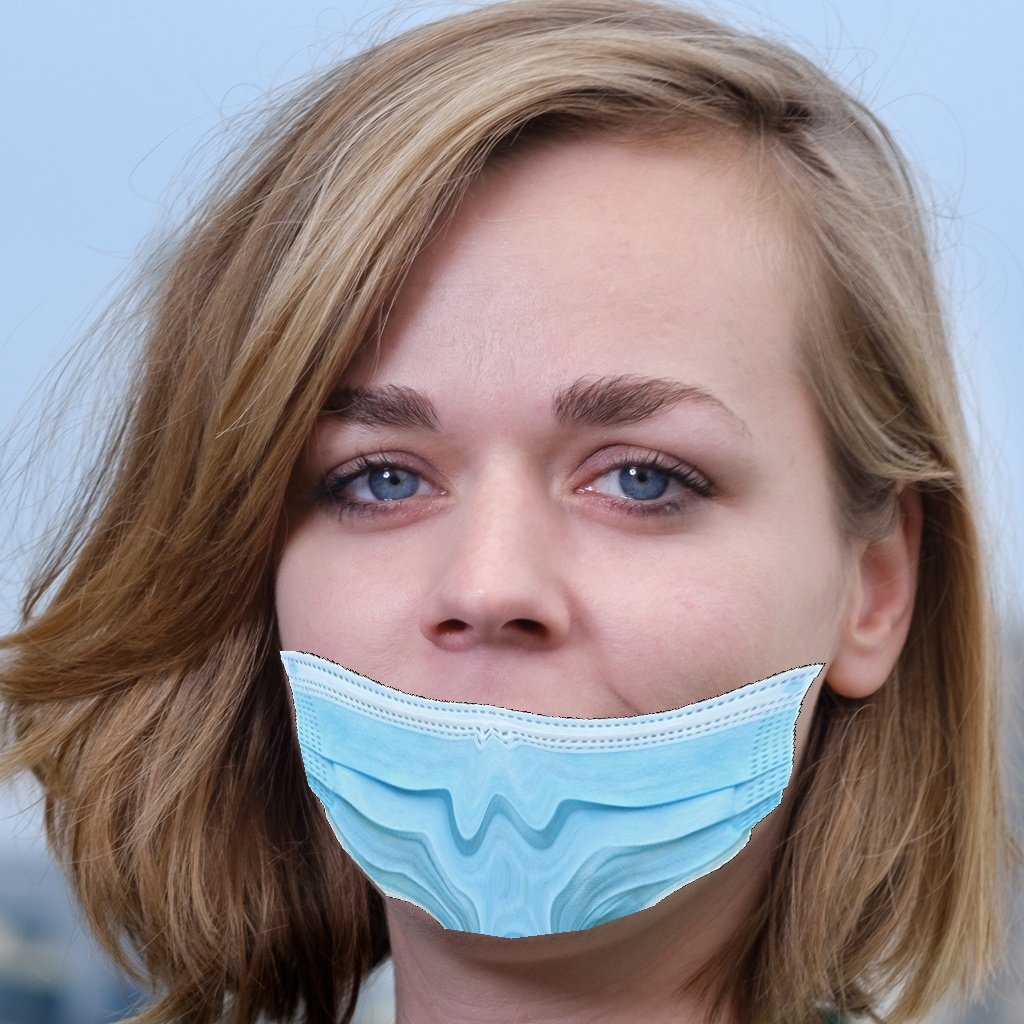
\includegraphics[width=\linewidth]{imagenes/dataset1-9.jpg}
		\caption{}
		\label{fig:1i}
	\end{subfigure}
	\caption{Ejemplos de imágenes del dataset 1 (\ref{fig:1a}, \ref{fig:1b}, \ref{fig:1d}, \ref{fig:1e}, \ref{fig:1f}, \ref{fig:1g}) y del dataset 2 (\ref{fig:1c}, \ref{fig:1h}, \ref{fig:1i}).}
	\label{fig:1}
\end{figure}




% Diseño y resolución
%!TEX root = proyecto.tex

\chapter{Diseño y resolución}

%\linespread{1.5}

\section{Paul Viola and Michael Jones} \label{haar-like}

En 2001, el reconocimiento facial tuvo su primera aparición en el campo de la visión artificial como aplicación en tiempo real. Este avance fue de la mano de Paul Viola y Michael Jones. Análogamente, el punto de partida del estudio de este TFG. Durante este apartado, se estudiará el funcionamiento del algoritmo \textit{Viola-Jones face detector}, ideado por estos dos investigadores y se realizará una implementación del mismo mediante \textit{Python} y \textit{OpenCV} para comprobar como se comporta en la situación actual.

\subsection*{Método de estudio}

El trabajo de los expertos fue presentado por parte de la Universidad de Cambridge mediante un \textit{paper} (ensayo de la investigación). Y se introduce como: 
\begin{quote}
	"[...] This paper describes a machine learning approach for visual object detection which is capable of processing images extremely rapidly and achieving high detection rates" \cite{paulViola}
\end{quote}

Para poder lograr esta afirmación se basan en un procedimiento de trabajo en dos fases: entrenamiento y detección. Igualmente, Paul y Michael dividen el proyecto en tres ideas principales para poder lograr un detector que se pueda ejecutar en tiempo real. Y estas son: la imagen integral, Adaboost (algoritmo de Machine Learning) y un método llamado \textit{attentional cascade structure}. 

Con todos estos puntos combinados lograron ingeniar un prototipo capaz de detectar caras humanas con un \textit{frame rate} de 15 fps. Fue diseñado para la detección de caras frontales, haciéndose difícil para posiciones laterales o inclinadas.

Las imágenes que se toman para realizar la detección pasan por una transformación del espacio de color a \textit{grayscale}. Con el objeto de encontrar características en ellas, llamadas \textit{haar-like features}. Nombradas así por su inventor Alfred Haar en el siglo XIX. En este trabajo se hacen uso de tres tipos de haar-like features (Figura \ref{fig:haarLike}).

\begin{figure}[htp]
	\centering
	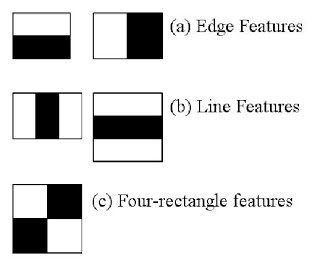
\includegraphics[width=5cm]{imagenes/haar-like.jpeg}
	\caption{Haar-like Features \cite{haar-like}.}
	\label{fig:haarLike}
\end{figure}

Las \textbf{\textit{Haar-like features}}, o también conocidas como \textit{Haar-wavelet} son una secuencia de funciones \textit{rescaled square-shaped}, siendo similares a las funciones de Fourier y con un comportamiento parecido a los \textit{Kernel} usados en las \textit{Redes Convolucionales} (matrices que consiguen extraer ciertas \textit{features} de la imagen de entrada). De manera que, las \textit{Haar Features} serán las características de la detección facial.

En un estudio ideal, los píxeles que forma el \textit{feature} tendrá una división clara entre píxeles de color blanco con los de color negro (Figura \ref{fig:haarLike}), pero en la realidad eso casi nunca se va a dar.

Más específicamente, las \textit{Haar-like features} están compuestas por valores escalares que representan la media de intensidades entre dos regiones rectangulares de la imagen. Estas capturan la intensidad del gradiente, la frecuencia espacial y las direcciones, mediante el cambio del tamaño, posición y forma de las regiones rectangulares basándose en la resolución que se define en el detector \cite{haar-like}. 

Estas características van a ayudar al ordenador a entender lo que es la imagen estudiada. Van a ser utilizadas mediante \textit{Machine Learning} para detectar donde hay una cara o no, mediante un recorrido sobre toda la imagen. Esto conlleva una potencia de computación elevada. Para paliar este problema idearon el método de la \textit{Imagen Integral}.

La \textbf{\textit{Imagen Integral}} permite calcular sumatorios sobre subregiones de la imagen, de una forma casi instantánea. Además de ser muy útiles para las \textit{HAAR-like features}, también lo son en muchas otras aplicaciones.

Si se supone una imagen con unas dimensiones de $<w,h>$ (ancho y alto, respectivamente), la imagen integral que la representa tendrá unas dimensiones de $<w+1,h+1>$. La primera fila y columna de esta son ceros, mientras que el resto tendrán el valor de la suma de todos los píxeles que le preceden \cite{integral-web}. Ahora, para calcular la suma de los píxeles en una región especifica de la imagen, se toma la correspondiente en la imagen integral y se suma según la siguiente fórmula (siguiendo la numeración de la Figura \ref{fig:integral}):
\begin{center}
	$sum = L4 + L1 - (L2 + L3)$ 
\end{center}
\begin{figure}[htp]
	\centering
	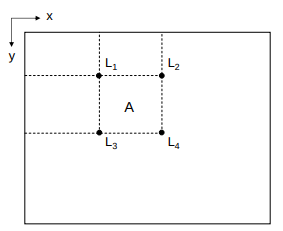
\includegraphics[width=5cm]{imagenes/integral.png}
	\caption{Funcionamiento de una \textit{Imagen Integral} \cite{integral-web}.}
	\label{fig:integral}
\end{figure}

Viola y Jones junta esta propuesta con los filtros \textit{Haar-like features}, y consiguen computar dichas características de manera constante y eficaz \cite{integral}.

% ---------------------------
%https://aishack.in/tutorials/integral-images-opencv/

%https://www.quora.com/How-integral-image-is-used-in-image-processing-and-how-improves-the-computation-time?share=1
%https://www.quora.com/What-are-the-must-read-papers-in-the-field-of-computer-vision-for-a-student-in-pursuing-research-in-the-field
% ---------------------------
%
% MACHINE LEARNING - ADABOOST
Una vez estudiada la obtención de características y con un set de entrenamiento, solo queda seleccionar un método de \textit{Machine Learning} que permita crear una función de clasificación. Concretamente, se plantea el uso de una variante de \textbf{\textit{AdaBoost}}, que permite seleccionar un pequeño conjunto de características y poder entrenar un clasificador. 

Este algoritmo de aprendizaje esta basado en generar una predicción muy buena a partir de la combinación de predicciones peores y más débiles, donde cada uno de estas se corresponde con el \textit{threshold} de una de las características \textit{Haar-like}. La primera vez que aparece este algoritmo, de forma práctica, fue de la mano de \textit{Freund y Schapire} \cite{adaboost1}. Sin embargo, el usado por \textit{Viola y Jones} es una modificación de este. La salida que genera el algoritmo \textbf{\textit{AdaBoost}} es un clasificador llamado \textit{Strong Classifier}, como se ha mencionado anteriormente, compuesto por combinaciones lineales de \textit{Weak Classifiers}. 

El procedimiento para encontrar \textit{Weak Classifiers} es ejecutar el algoritmo T iteraciones donde T es el número de clasificadores a encontrar. En cada iteración, el algoritmo busca el porcentaje de error entre todas las características y escoge la que menos porcentaje de error presente en dicha iteración \cite{adaboost2}. (Como se muestra en la \textit{Figura \ref{fig:ada1}}) 

\begin{figure}[htp]
	\centering
	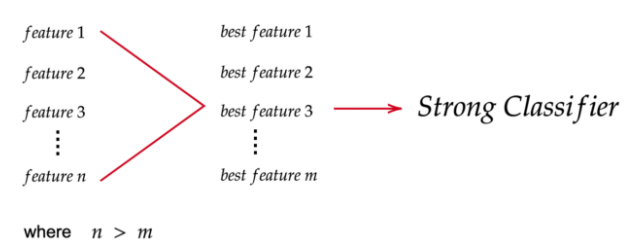
\includegraphics[width=10cm]{imagenes/ada1.png}
	\caption{Construcción del \textit{Strong Classifier} \cite{adaboost2}.}
	\label{fig:ada1}
\end{figure}

Con estos clasificadores se procede a la construcción de una estructura en cascada para crear un \textit{Multi-stage Classifier}, que podrá realizar una detección rápida y buena. Por tanto, la estructura de cascada esta compuesta por varios estados de \textit{Strong Classifiers} generados por el algoritmo \textit{AdaBoost}. Donde el trabajo de cada estado será identificar si, dada una región de la imagen, no hay una cara o si hay la posibilidad de que la haya \cite{adaboost1}. Si el resultado de uno de los estados es que no existe una cara en dicha región, esta se descarta directamente. Mientras que, si hay la posibilidad de que exista una, pasa al siguiente estado de la estructura. De tal forma que, cuantos más estados atraviese una región de la imagen, con más seguridad se podrá afirmar que existe una cara en ella. La estructura completa se refleja en la \textit{Figura \ref{fig:ada2}}.

\begin{figure}[htp]
	\centering
	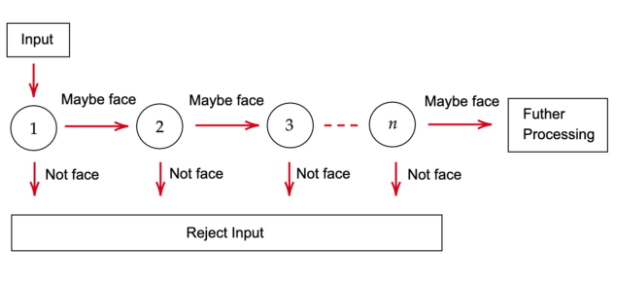
\includegraphics[width=8cm]{imagenes/ada2.png}
	\caption{Construcción del \textit{Multi-stage Classifier} \cite{adaboost2}.}
	\label{fig:ada2}
\end{figure}

% VIDEO DE LOCOS: https://www.youtube.com/watch?v=uEJ71VlUmMQ&t=5s

\subsection*{Implementación y Experimentación}

El prototipo será implementado en \textit{Python}, con el uso de \textit{OpenCV}. Y, el objetivo es construir dos detectores de caras, donde el primero usará dos modelos preentrenados de \textit{OpenCV} de caras frontales, para estudiar cual es mejor para el siguiente prototipo. Mientras que en el segundo, se intentará modificar el programa, para que mediante el uso de uno de estos modelos preentrenados y uno de \textit{Machine learning} se pueda detectar una cara con una mascarilla o sin ella.

La \textbf{implementación básica} hace uso de un modelo preentrenado cargado mediante una clase de \textit{OpenCV}, llamada \textit{Cascade Classifier}. Esta representa la base de \textit{Machine Learning} explicado en el apartado anterior. Asimismo, \textit{OpenCV} también proporciona una serie de archivos \textit{xml} con diferente modelos preentrenados. En concreto, para este prototipo se hace uso del modelo por defecto, detector de caras frontal, como se muestra en la investigación de \textit{Viola y Jones}, y una variante del mismo denominada \textit{frontalface\_alt2.xml}. Finalmente, la detección se realiza, tras hacer una transformación del espacio de color a blanco y negro, mediante la función \textit{detectMultiScale} de la clase, creada anteriormente, \textit{Cascade Classifier}. Concretamente, su funcionalidad será encontrar caras dentro de las imágenes que vaya procesando.

La prueba de esta prototipo se realizará a una distancia corta (70 cm)  y media (150 cm), para comprobar su funcionamiento estandar con dos modelos pre-entrenados, llamados:  \textit{frontalface\_default.xml} y \textit{frontalface\_alt2.xml}, dedicados a reconocer rostros de manera frontal. Intentando estudiar su velocidad de procesamiento y su precisión a la hora de detectar un rostro sin y con obstáculos, el resultado obtenido se ve reflejado en la \textit{Figura \ref{fig:haar1}}.

\begin{figure}[htp]
	\centering
	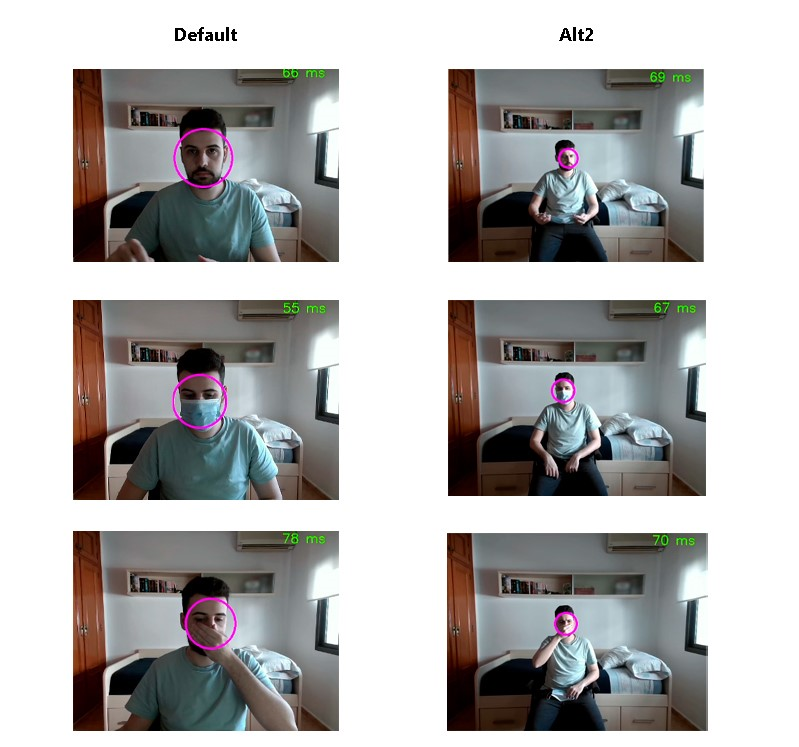
\includegraphics[width=10cm]{imagenes/prueba_proto1.jpg}
	\caption{Pruebas con Haar-like features con: \textit{frontalface\_default.xml} y \textit{frontalface\_alt2.xml}}
	\label{fig:haar1}
\end{figure}

Tras la experimentación se puede comprobar que ambos modelos funcionan bastante bien, tanto para un reconocimiento de rostro sin obstáculos como con ellos. Aunque, es importante destacar que el modelo pre-entrenado \textit{frontalface\_default.xml} no es tan preciso en distancias superiores a los 150 cm. En cuanto a los tiempos recogidos para estas pruebas, el segundo modelo pre-entrenado \textit{frontalface\_alt2.xml} obtiene un tiempo medio más lento pero funciona de forma más precias. Se refleja en la siguiente tabla:

\begin{table}[h!]
	\begin{center}
		\begin{tabular}{ |c|c|c|c|c|c| } 
			\hline
			& default (70cm) & default (150cm) & alt2 (70cm) & alt2 (150cm) \\
			\hline
			PC1 / Time (MS) & 46.15  & 45.09 & 62.04  & 61.75 \\
			\hline
			PC2 / Time (MS) & X  & X & X  & X \\
			\hline
		\end{tabular}
		\caption{Tiempos para el prototipo 1.}
		\label{tab:table2}
	\end{center}
\end{table}

El \textbf{segundo prototipo} (custom) implementa un identificador de caras conjunto a un modelo de \textit{Machine Learning} que identifica cuando una persona lleva o no mascarilla, además de si se lleva bien. Gracias a los modelos PCA y SVM, se puede crear un modelo para su identificación con el uso de muestras de los modelos pre-entrenados \textit{Haar-like features} probados antes. Para ello se realizará el siguiente esquema de procedimiento:

\begin{enumerate}
	\item Haar-like features
	
	Sigue el mismo procedimiento que el prototipo anterior. Mediante la creación de una clase de OpenCV, llamada \textit{CascadeClassifier}, y el uso de un modelo \textit{Haar-like features} pre-entrenado, se obtiene el ROI donde se localiza un rostro. En este caso, se hará un estudio con el modelo pre-entrenado llamado \textit{frontalface\_alt2.xml}, capaz de reconocer de forma más fiable rostros con mascarilla. 
	
	\item Modelo PCA/SVM
	
	Una vez obtenido el ROI de la localización de la cara con o sin mascarilla, se procede a predecir de que caso se trata. Previo a dicha predicción y ejecución del prototipo, se necesita entrenar el modelo. Y para ello se toman referencias de rostros con y sin la mascarilla para que sirvan como entrada en el entrenamiento del modelo, usando el prototipo anterior. Exactamente se debe ejecutar dos veces el archivo \textit{Python: trainCascade.py}, una para el caso de sin y otro para el caso de con mascarilla. Siendo la mejor opción, el uso del modelo pre-entrenado \textit{frontalface\_alt2.xml}. También es posible realizar el entrenamiento con imágenes de un dataset.
	
	Principal Component Analysis, (\textbf{PCA}), es un algoritmo de \textit{Machine Learning} dedicado a la reducibilidad de dimensionalidad. Identifica un hiperplano común que conecta a todos los datos y son proyectados sobre él. \textit{Scikit-Learn} ofrece una implementación de este, mediante descomposición SVD (Singular Value Decomposition), también conocido como una regresión lineal \cite{geron_2020}. La salida de PCA servirá para reducir la complejidad de la entrada al modelo \textbf{SVM} (Support Vector Machine), capaz de realizar regresiones o clasificaciones tanto lineales como no lineales. La idea tras este modelo es separar los distintos conjuntos de datos existentes mediante lineas rectas en el espacio (Figura \ref{fig:svm}) \cite{geron_2020}.
	
	\begin{figure}[htp]
		\centering
		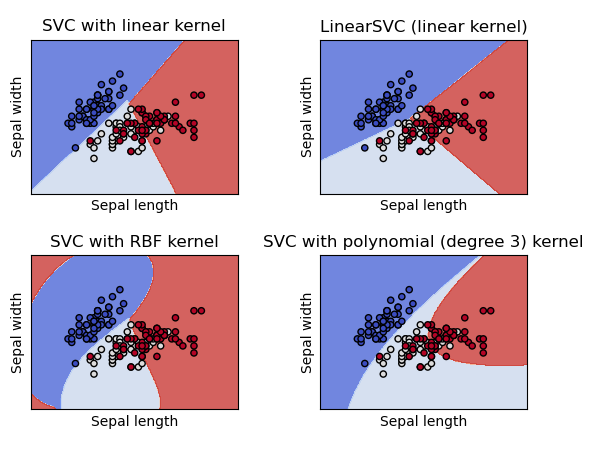
\includegraphics[width=7cm]{imagenes/svm_example.png}
		\caption{Ejemplos de clasificaciones SVM}
		\label{fig:svm}
	\end{figure}

	Para la implementación de esta parte se hace uso de \textit{Scikit-Learn}, librería de Python que implementa una gran variedad de clasificadores, regresores y cluster de modelos \textit{Machine Learning}.
\end{enumerate}

En resumen, el procedeminiento que sigue este prototipo se basa en cargar el modelo que se ha creado, detectar un rostro en al imagen de entrada y a partir de ese ROI (donde se encuentra dicho rostro), hacer un estudio con el modelo y mostrar por pantalla el resultado. Para la detección de los rostros antes de tratarlos con el modelo se realizará con el modelo pre-entrenado \textit{frontalface\_default.xml}, para conseguir un funcionamiento más fluido. El funcionamiento del prototipo se muestra en la Figura \ref{fig:haarCustom}.

\begin{figure}[htp]
	\centering
	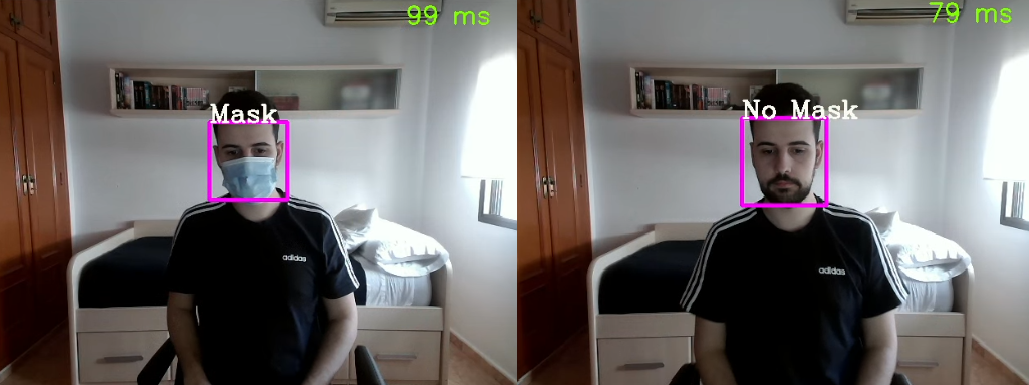
\includegraphics[width=15cm]{imagenes/haarcustom_prueba.png}
	\caption{Pruebas con prototipo Haar Custom}
	\label{fig:haarCustom}
\end{figure}

La desventaja es que solamente funciona con los rostros/rostro que se toma como referencia para construir el modelo, igualmente pasa con el tipo de mascarilla (siendo la quirúrgica la que mejor funciona con este prototipo). Asimismo, su funcionamiento es de manera frontal y cercana, tanto a 70 cm como a 150 cm, funciona de forma correcta. Sin embargo, para una posición lejana y con más información a tratar el detector se pierde y crea identificaciones falsa o no llega a reconocer nada. Asimismo, el tiempo de retardo que presenta este prototipo para el PC1 es de una media de 87.5 ms.

Este procedimiento se podría llegar a usar con otra implementación, específicamente con HOG, centrada también en la extracción de caracteristicas pero usando gradientes.

\newpage
\section{Facial Landmark}

Con el objetivo de ampliar la idea anterior, se plantea el uso de Facial Landmark, una tecnología que nos permite el reconocimiento de puntos de interés en las caras que se han detectado en la imagen. Sus pasos de ejecución son: detectar cara dentro de la imagen (En este caso, se usará \textit{Haar-like features}) y obtener dichos puntos de interés. La implementación que se va a utilizar es la estudiada por \textit{Kazemi} y \textit{Sullivan} en 2014, con el paper \textit{One Millisecond Face Alignment with an Ensemble of Regression Trees} \cite{inproceedings}, y usado en el \textit{toolkit} \textit{Dlib}. Este método se centra en localizar las siguientes zonas faciales: boca, cejas, ojos, nariz y mentón, gracias al uso de un conjunto de árboles de regresión. Estos son entrenados mediante  un modelo formado por puntos de interés de un grupo de imágenes, etiquetados a mano y especificadas como coordenadas (x,y). 

\textit{Dlib} será el \textit{toolkit} (\textit{Open Source}) utilizado para la implementación de dicho método. Este contiene algoritmos de \textit{Machine Learning} y herramientas capaces de crear software complejo en \textit{C++} y \textit{Python} para resolver problemas reales. Sobre todo centrado en robótica, dispositivos embebidos, móviles y ordenadores de gran capacidad \cite{dlib}. 

\subsection*{HOG - \textit{Histogram of Oriented Gradients}}

El primer paso en esta solución es encontrar una cara dentro de la imagen de entrada, y el encargado será el método HOG. El cual, sigue una idea similar al método de \textit{Haar-like}, ya que se basa en la detección de \textit{features} (características).

La idea teórica tras \textit{HOG} es encontrar la apariencia y forma de un objeto mediante la distribución de la intensidad de gradientes locales, gracias a que estos obtienen una magnitud mayor en las cercanías de bordes o esquinas. Mientras que la implementación, divide la imagen en pequeñas regiones (llamadas celdas) y se calcula un histograma de gradientes de una dimensión para cada uno de los píxeles de cada celda. Para un mejor estudio se normaliza el contraste de la imagen de entrada \cite{hog}. Con este procedimiento se obtiene un \textit{feature vector} a partir de la imagen de entrada, y la distribución resultante de los gradientes serán usados como las características. La implementación de HOG se podría dividir en 5 pasos generales \cite{hog2}:

\begin{enumerate}
	\item \textit{Pre-procesado}: Para una imagen de entrada de cualquier tamaño es tratada en regiones de ciertas escalas y analizadas en varias zonas de la imagen. La única restricción es que los tamaño de las regiones analizadas tienen una relación de aspecto fija.
	
	\item \textit{Cálculo de las imágenes de gradiente}: Para el calculo del histograma de gradientes es necesario realizar el cálculo de los gradientes, tanto verticales como horizontales. Esto se puede obtener fácilmente gracias al uso de \textit{Kernels} (filtros). Posteriormente, se busca la magnitud de las direcciones de dichos gradientes con el uso de la siguiente fórmula (Figura \ref{fig:hogf}):
	
	\begin{figure}[htp]
		\centering
		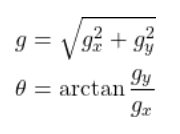
\includegraphics[width=3cm]{imagenes/HOGFormula.png}
		\caption{Fórmula \textit{HOG} \cite{hog2}.}
		\label{fig:hogf}
	\end{figure}
	
	La fórmula esta implementada en \textit{OpenCV} mediante la función \textit{cartToPolar}. En este punto se puede obtener la imagen de los gradientes, eliminando toda la información no relevante de la imagen original, observando como en todos los píxeles el gradiente tomarán una magnitud y una dirección. Si la imagen es RGB, los gradientes se evalúan sobre los tres canales de color, siendo la magnitud final el valor mayor entre los tres canales.
	
	\item \textit{Cálculo de los histogramas de gradientes en celdas (8x8)}: La imagen se divide en celdas y se calculan los histogramas para cada una de ellas. Por ejemplo, si la celda es de tamaño 8x8, esta contendrá 192 píxeles (8x8x3), donde el gradiente tiene dos valores, descritos anteriormente (magnitud y dirección), por cada uno de los píxeles, lo que añade 128 valores (8x8x2). Esto facilita la representación de las regiones mediante el uso de un histograma, además mejora la influencia al ruido. El tamaño de la celda vendrá definida dependiendo de la escala de características (\textit{features}) que se estén buscando.
	
	\item \textit{Normalización de bloques (16x16)}: Una vez creado el histograma, hay que tener en cuenta que la imagen es sensible al brillo que tenga. Por ejemplo, si el brillo de la imagen se divide en dos, la magnitud del gradiente también lo hará. De igual forma, si el brillo se multiplica por dos, el gradiente ídem. Pero, se busca un descriptor que sea independiente a esto, por lo que se normaliza el histograma para que no se vea afectado por los cambios de luz/brillo.	Disponiendo de celdas de 8x8, un bloque de 16x16 posee cuatro histogramas que pueden ser condensados en un único vector normalizado.
	
	\item \textit{Cálculo del vector de HOG}: El último paso es concatenar los vectores normalizados obtenidos en uno global.

\end{enumerate}

Este procedimiento se repite varias veces sobre imágenes distintas y se introduce en un modelo \textit{Machine Learning} del tipo SVM Linear, con el objetivo de obtener un detector de caras. En el caso de \textit{Dlib}, posee un modelo preentrenado.


\subsection*{Sullivan Paper}

El \textit{paper} de Kazemi y Sullivan presenta la implementación usada en el \textit{toolkit Dlib} del algoritmo que estima de forma precisa y eficiente los puntos de interés faciales. Esta basado en \textit{gradient boosting} para el aprendizaje de un conjunto de arboles de regresión (\textit{ensemble of regression trees}), que será el encargado de la predicción de los puntos de interés \cite{faceLandmark}.

Este método fue uno de los primeros que mejoró el rendimiento, a diferencia con los métodos anteriores, gracias a la detección de componentes esenciales para el \textit{face aligment} y procesarlos para introducirlos en funciones de regresión en cascada. Cada una de estas funciones estima, de forma eficiente, la forma facial desde una estimación inicial y obtiene un conjunto de píxeles indexados a dicha estimación. En concreto, \textit{Dlib} estimará un total de 68 píxeles indexados (Figura \ref{fig:dlibPoints}), ya que sigue las anotaciones del \textit{dataset iBUG 300-W} \cite{ibug}, usado en los modelos pre-entrenados ofrecidos por \textit{Dlib}.

\begin{figure}[htp]
	\centering
	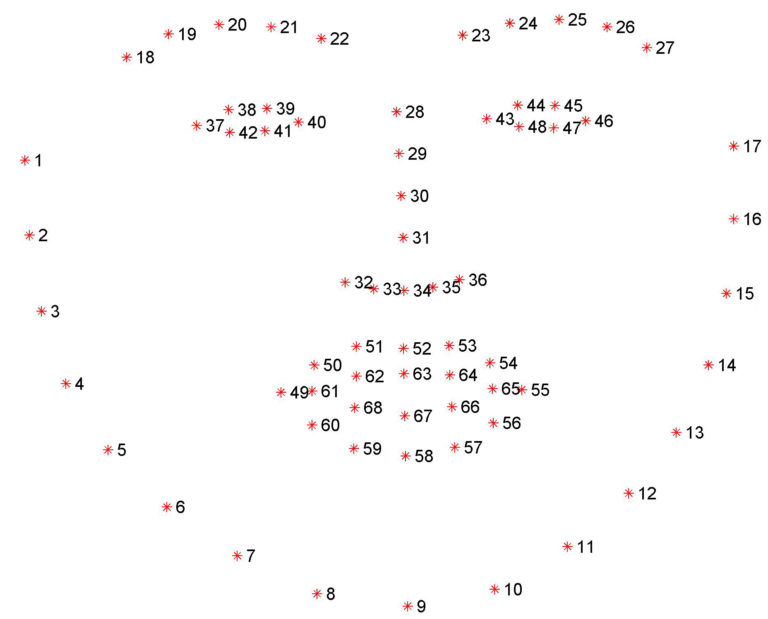
\includegraphics[width=8cm]{imagenes/facial_landmarks_68markup.jpg}
	\caption{68 coordenadas del \textit{facial landmark} con \textit{iBUG 300-W} \textit{dataset} \cite{ibug}.}
	\label{fig:dlibPoints}
\end{figure}

Además, se introdujeron dos elementos clave a las funciones de aprendizaje de regresión. El primero gira en torno a la intensidad de los píxeles indexados con respecto a la estimación actual de la forma facial, ya que estos son muy influenciables por la deformación de la estimación de la forma y a los cambios de iluminación. El dilema que aparece es que necesitamos características confiables para obtener una predicción con precisión la forma y, por otro lado, necesitamos una estimación precisa de la forma para extraer características fiables. Para resolver este dilema se plantea el uso de un enfoque iterativo. La idea se basa en obtener una imagen transformada en un sistema de coordenadas normalizado basado en una estimación actual de la forma, y posteriormente extraer las características para predecir un vector de actualización para los parámetros de la forma. Este proceso suele repetirse varias veces.

El segundo elemento clave se trata de reducir la dificultad del proceso de inferencia/predicción. El objetivo es obtener una función capaz de estimar la forma que concuerde con la información de la imagen y el modelo. 
%Pero el problema es que esta función es no convexa en varios valores locales.
Para resolver esto se plantearon dos soluciones a lo largo del tiempo. El primero afirma que las predicciones estimadas en zonas lineales del subespacio mienten, lo que concluyo siendo de ayuda para evitar este problema. Pero, posteriormente se descubrió una segunda solución, donde se asume que la función miente en zonas lineales del subespacio pero no es necesario realizar trabajo adicional. En el caso de este \textit{paper}, se implementa una solución donde se utilizan una combinación de ambas. Por lo que, cada regresor aprende mediante \textit{gradient boosting} conjuntamente a una función de perdida de error al cuadrado.
%La entrada usada en el regresor, es seleccionada mediante \textit{gradient boosting} sobre un conjunto de píxeles dispersos, y la prioridad de probabilidad sobre la distancia entre pares de píxeles de entrada. 
Esto permite realizar un estudio sobre un mayor número de características relevante de forma eficiente. El resultado es una cascada de regresores que pueden localizar los puntos de referencia faciales cuando es inicializada con la media de la pose facial \cite{faceLandmark}.

\newpage
De forma más general, la investigación ofrece las siguiente contribuciones a las investigaciones de \textit{Face Landmark} anteriores:

\begin{enumerate}
	\vspace{-0.2cm}
	\item Un método de alineación basado en un conjunto de árboles de regresión que devuelve la forma facial mientras minimiza la función de error.
	\vspace{-0.2cm}
	\item Método que maneja la predicción de puntos que faltan o no están presentes en la imagen. Por ejemplo, rostros que estén medio ocultos. (Esto solamente se realizará si el modelo creado con HOG detecta dicha cara oculta).
	\vspace{-0.2cm}
	\item Resultados donde se demuestran que el método produce predicciones de alta calidad.
	\vspace{-0.2cm}
	\item El efecto de la cantidad de datos de entrenamiento.
\end{enumerate}

\vspace{-0.8cm}
\subsection*{Prototipo}
\vspace{-0.5cm}
Mediante \textit{OpenCV} y el \textit{ToolKit Dlib} se obtiene la implementación de ambas ideas, mediante modelos pre-entrenados. Para la detección facial y predicción de puntos de interés se realizará el uso de los modelos propuesto por Dlib, siendo el de detección basado en HOG y el de predicción llamado \textit{shape\_predictor\_68\_face\_landmarks.dat}. El procedimiento que seguirá este prototipo será el siguiente:

\begin{enumerate}
	\item Detección facial: Dlib dispone de una función donde inicializa un detector basado en HOG con el que se podrá determinar donde se encuentra el rostro en la imagen. Para realizar la detección tiene que recibir una imagen transformada en el espacio de color \textit{GRAY}.
	\item Predicción de \textit{Facial Landmarks}: Una vez detectados los rostros de la imagen, se utiliza un predictor creado con la función \textit{shape\_predictor} de Dlib. Este es capaz de determinar los puntos de interés de un ROI con el rostro detectado anteriormente. En este punto es necesario el uso de un modelo pre-entrenado, exactamente el de 68 puntos de interés (nombrado anteriormente).
	\item Se obtiene el ROI de la zona donde se encuentra la boca, a través de los puntos de interés obtenidos en el paso anterior.
	\item Detección de una boca dentro del ROI: Mediante un modelo pre-entrenado y basándonos en el prototipo anterior de \textit{Haar-like features} se construye un detector capaz de detectar una boca. Con el objetivo de que si se detecta una boca se puede decir que la persona no lleva mascarilla, mientras que, si no es capaz de realizar una detección si que llevaría mascarilla.
\end{enumerate}

\begin{figure}[htp]
	\centering
	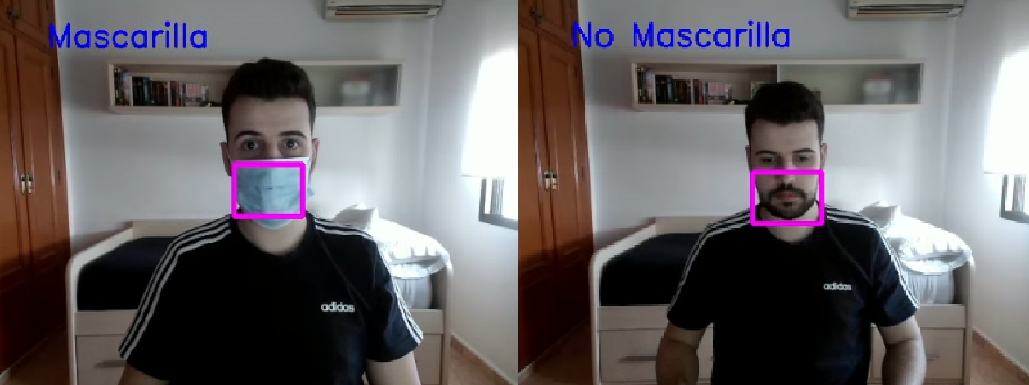
\includegraphics[width=12cm]{imagenes/landmark_prueba.png}
	\caption{Pruebas con Dlib's Facial Landmarks y modelo Haar-like feature \textit{mcs\_mouth.xml}.}
	\label{fig:dlibLandmarks}
\end{figure}

El tiempo de retardo que presenta este prototipo para el PC1 es de una media de 14,7 ms. Aunque estos tiempos presenten un buen resultado, el funcionamiento del prototipo no es el esperado. Por un lado, le cuesta reconocer un rostro con mascarilla, incluso en muchas ocasiones sin lograrlo, ya en el primer tipo de prueba (distancia de 75 cm). Por otro lado, el detector facial sin mascarilla funciona correctamente y de manera eficaz (Figura \ref{fig:dlibLandmarks}). Por lo que, otro planteamiento que se podría desarrollar sería un prototipo donde si aparece una detección de una persona y su boca significa que no viste una mascarilla, por tanto no cumpliría con la normativa y saltaría la alarma.

\vspace{-0.8cm}
\subsection*{Próximos pasos}
\vspace{-0.5cm}
En los siguientes apartados se probará implementar prototipos con el uso de Deep Learning. En las últimas décadas, se ha convertido en uno de los métodos mas usados para la creación de aplicaciones de visión artificial. \cite{szeliski_2018}. Esta basado en las estructuras neuronales CNN (\textit{Convolutional Neural Network}), principales responsables de que un ordenador pueda procesar de forma sencilla una imagen. \textit{CNN} es una combinación entre capas neuronales y convolucionales, siendo estas últimas filtros con los que se obtendrán características de la imagen de entrada, los conocidos \textit{features}. La principal función del Deep Learning es clasificar, ya sea una imagen, un objeto o incluso varios objetos a la vez. Esto es gracias al uso de modelos, entrenados con miles de imágenes, que consiguen clasificar imágenes en varias categorías, por ejemplo \textit{MobileNet} \cite{cnn}. 

\newpage
\section{Mediapipe}

Mediapipe es una API \textit{open-source} creada por \textit{Google}, que ofrece servicios de \textit{Machine Learning} para vídeos y fuentes multimedia. Entre ellas, se encuentra un servicio llamado \textit{Face Mesh} que ofrece una solución que estima 468 puntos de interés de un rostro, conformando una malla 3D en tiempo real. Este usa aceleración GPU conjuntamente con un modelo y el uso de una \textit{pipeline}.

La \textit{pipeline} que se utiliza en esta API consiste en dos modelos de \textit{Deep Learning} que trabajan al mismo tiempo. Su funcionalidad es realizar una detección a partir de una imagen de los puntos de interés sobre una cara y construir un modelo \textit{face landmark} 3D que aproxima la superficie de esta mediante regresión sobre dichos puntos. Esta tarea es facilitada si la cara, donde se tienen que detectar los puntos de interés, se encuentra recortada, haciendo así que el modelo se centre solamente en buscar los puntos, aumentando la precisión de la predicción. Asimismo, los recortes de las caras se puede generar a partir de las predicciones anteriores realizadas por el mismo modelo, y solamente es llamada la predicción nuevamente cuando no se consigue detectar la presencia de la cara \cite{faceMesh}.

Todo esto es implementado gracias al framework \textit{MediaPipe}, con la herramienta \textit{MediaPipe graph}. Arquitectura caracterizada por estar formada por componentes llamados \textit{Calculator}, nodos del grafo que tras la entrada de cero o más inputs generan cero o más salidas. Todos estos nodos están conectados mediante datos en forma de \textit{Streams}, donde cada uno representa un conjunto de datos-tiempo en \textit{Packets}. Por tanto, los \textit{calculators} y \textit{steams} definen el flujo de datos del \textit{Graph} \cite{mediapipe}. 

El \textit{pipeline} puede ser definido mediante la adición/modificación de \textit{calculators} dentro del \textit{graph}. Específicamente, el \textit{pipeline} que se utiliza en esta solución (\textit{FaceMesh}) esta formada por un \textit{graph} compuesto por un \textit{subgraph} de \textit{face landmark} (proveniente del módulo, ya implementado, de \textit{face landmark} de \textit{Mediapipe}), donde a su vez usa otro \textit{subgraph} proveniente de \textit{face detection module} para la detección de caras, y un \textit{face renderer subgraph} para mostrar el resultado \cite{faceMesh}. En concreto el \textit{graph} que se usa en esta implementación es el mostrado en la Figura \ref{fig:faceMesh}.

\begin{figure}[htp]
	\centering
	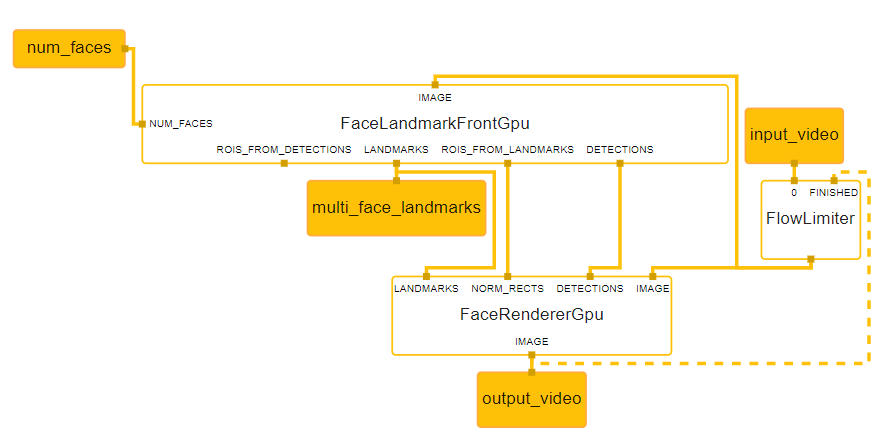
\includegraphics[width=10cm]{imagenes/faceMesh.png}
	\caption{MediaPipe Graph utilizado en FaceMesh \cite{mpGraph}.}
	\label{fig:faceMesh}
\end{figure}

Por tanto, el procesamiento de una imagen en este modelo sigue dos pasos. El primero (1) toma la imagen de entrada, capturada por la cámara, es procesada por un detector de caras \textit{lightweigth}, llamado \textit{BlazeFace}, y produce unos rectángulos que definen el perímetro donde se encuentra la cara, conjuntamente con un par de puntos de interés superficiales (ojos, boca y nariz). Estos puntos se utilizarán para alinear la cara para el siguiente paso. Y el segundo (2), mediante el rectángulo obtenido en el paso anterior, se recorta la cara de la imagen inicial y es re-escalado para utilizarse como entrada de la red neuronal que realiza la predicción de la malla. (El tamaño de re-escalado será entre 256x256 en un modelo completo, hasta 128x128 en el modelo más pequeño). Tras la predicción, se obtiene como salida un vector de coordenadas \textit{landmark 3D}, que serán mapeadas y dibujadas en la imagen original \cite{faceMesh2}. 

Las coordenadas que se obtienen como salida están compuestas por unas coordenadas x e y provenientes de localizaciones del plano 2D propio de la imagen. Mientras que, la coordenada z es interpretada como una profundidad relativa a un centro de masa que compone la malla de la cara.

Se utilizan dos modelos para el funcionamiento de \textit{FaceMesh}. El primero de ellos dedicado a la detección facial, llamado BlazeFace (mencionado anteriormente). Modelo \textit{lightweight} creado para GPU móviles, llegando a una velocidad de procesamiento entre 200 a 1000 fps en dispositivos móviles punteros. Es inspirado en los modelos \textit{MobileNet}, tanto la primera versión como la segunda, provenientes del \textit{framework} SSD (\textit{Single Shot Multibox Detector}). Este modelo produce una salida compuesta por un rectángulo perimetral y 6 puntos de interés faciales. \cite{blazeface}

El segundo modelo, \textit{Face Landmark Model}, generado mediante \textit{Transfer Learning} buscando los siguientes objetivos: crear coordenadas 3D (mencionadas anteriormente) y conseguir mostrarlas en la imagen de salida de forma correcta \cite{faceMesh}. El \textit{Transfer Learning} es una técnica de \textit{Machine Learning} donde se puede hacer uso de un modelo pre-entrenado para personalizarlo y usarlo en una tarea determinada. Conviene destacar que un modelo entrenado es una red almacenada, entrenada previamente con un conjunto de datos con el objetivo de realizar una tarea de clasificación de imágenes a gran escala \cite{transferLearning}.

\textit{FaceMesh} propone una implementación mediante \textit{TensorFlow Lite} que dispone de dos formatos: CPU y GPU, que presentan un rendimiento en dispositivos móviles (\textit{Pixel3}, \textit{Pixel2} y \textit{iPhoneX}) muy fluido, impresionando sobre todo su funcionamiento sobre CPU. (Figura \ref{fig:faceMeshRen}) \cite{faceMesh3}.

\begin{figure}[htp]
	\centering
	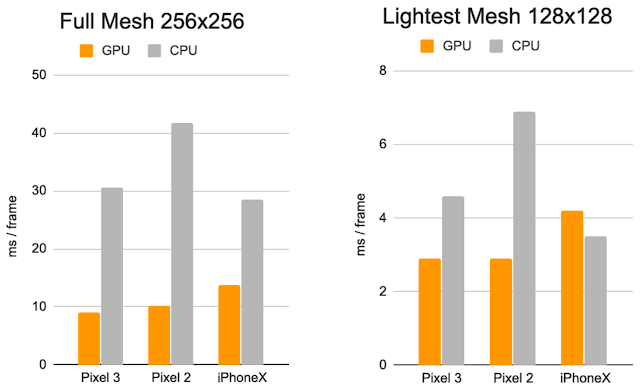
\includegraphics[width=10cm]{imagenes/rendFaceMesh.png}
	\caption{Rendimiento de FaceMesh sobre dispositivos móviles \cite{faceMesh3}.}
	\label{fig:faceMeshRen}
\end{figure}

\vspace{-0.8cm}
\subsection*{Prototipo}
\vspace{-0.5cm}
El prototipo de este apartado se realizará mediante el uso de \textit{FaceMesh} del framework \textit{MediaPipe} y un detector basado en \textit{Haar-like features}, como el mencionado en el \textit{paper} de Viola \& Jones (\ref{haar-like}). Los pasos que lo definen son los siguientes:

\vspace{-0.5cm}
\subsubsection*{1. Detección FaceMesh}
\vspace{-0.7cm}
Para la detección del rostro en la imagen de entrada se utiliza la solución de Mediapipe llamada FaceMesh, implementada en el framework de Python que recibe el mismo nombre, \textit{mediapipe}. Esta solución dispone de dos parámetros de configuración: \textit{min\_detection\_confidence} y \textit{min\_tracking\_confidence}. El primero hace referencia a ..., mientras que el segundo se entiende como ....

Una vez configurado el FaceMesh, se procede a tratar la imagen de entrada para facilitar su tratamiento. Se convierte el espacio de color de la imagen de BGR, espacio de color con el que trabaja \textit{OpenCV}, a RGB. Y, para mejorar el rendimiento, se elimina la opción de la imagen para que sea escribible (\textit{writeable}). Este proceso será invertido después de realizar la detección.

\begin{enumerate}
	\item Detección FaceMesh
	
	Para la detección del rostro en la imagen de entrada se utiliza la solución de Mediapipe llamada FaceMesh, implementada en el framework de Python que recibe el mismo nombre, \textit{mediapipe}. Esta solución dispone de dos parámetros de configuración: \textit{min\_detection\_confidence} y \textit{min\_tracking\_confidence}. El primero hace referencia a ..., mientras que el segundo se entiende como ....
	
	Una vez configurado el FaceMesh, se procede a tratar la imagen de entrada para facilitar su tratamiento. Se convierte el espacio de color de la imagen de BGR, espacio de color con el que trabaja \textit{OpenCV}, a RGB. Y, para mejorar el rendimiento, se elimina la opción de la imagen para que sea escribible (\textit{writeable}). Este proceso será invertido después de realizar la detección.
	
	\item Obtención de zona ROI
	
	Tras la detección de Landmarks, el resultado se almacena en una variable llamada \textit{multi\_face\_landmarks}, donde se encuentran todas las marcas faciales de todos los rostros detectados. A su vez, este contiene cada una de las marcas, con una totalidad de 468 puntos.

	Estas marcas contienen parámetros para medir la precisión de la detección del mismo, llamados: \textit{visibility} y \textit{presence}. Si estos valores son muy bajos no se tienen en cuenta. Tras esto, se normalizan sus valores a coordenadas con respecto a los píxeles de la imagen de entrada, se reservan unicamente las coordenadas relacionadas con la boca y se obtiene el ROI donde se localiza esta.
	
	\item Detección de una boca en el ROI 
	
	Para el último paso se hace uso de un modelo pre-entrenado de \textit{Haar-like features} llamado \textit{mcs\_mouth.xml}, capaz de detectar una boca. Si dentro del ROI no se detecta nada, significa que la persona tiene una mascarilla puesta.
\end{enumerate}

Por tanto, la idea tras este prototipo es obtener la zona de la boca gracias al uso de la solución proporcionada por Mediapipe, \textit{FaceMesh}. Y, posteriormente detectar mediante un modelo Haar-like features si existe una boca en dicha zona. Se utiliza la misma idea planteada en el prototipo anterior, pero intentando mejorar su funcionamiento con el uso del framework \textit{Mediapipe}. La desventajas de este prototipo es que si la persona obstaculiza la zona de la boca a la hora de la detección, podría ser capaz de engañar al algoritmo haciendo pensar que si porta una mascarilla, cuando en realidad no es así. Lo bueno es que no hace falta distinguir entre tipos mascarillas.

\begin{figure}[htp]
	\centering
	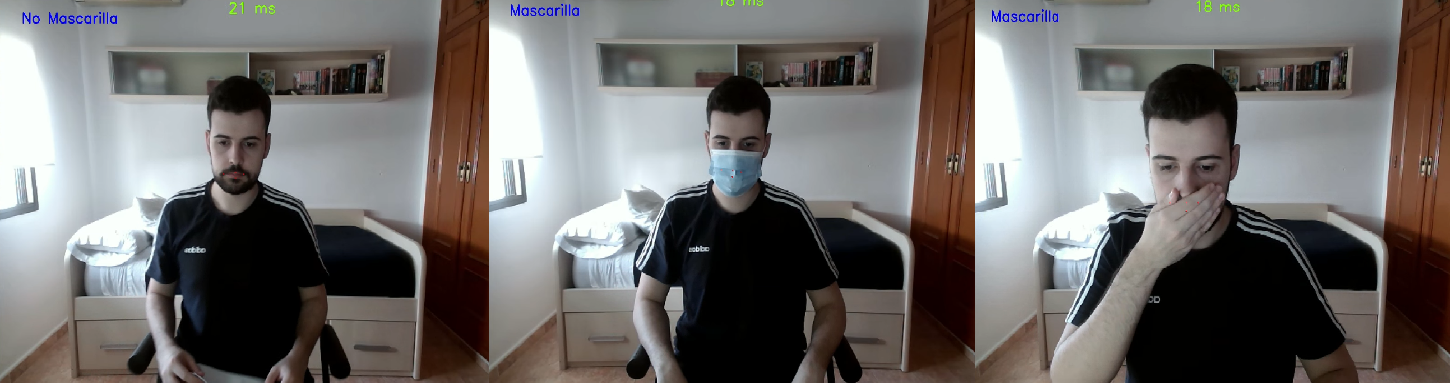
\includegraphics[width=17cm]{imagenes/mediapipe_prueba.png}
	\caption{Pruebas con Mediapipe FaceMesh y modelo Haar-like feature \textit{mcs\_mouth.xml}}
	\label{fig:protoMediapipe}
\end{figure}

El tiempo de retardo que presenta este prototipo para el PC1 es de una media de 12,3 ms. Tras la realización de las pruebas (Figura \ref{fig:protoMediapipe}), se puede concluir en que el prototipo funciona de una manera bastante eficaz y precisa en distancias cercanas, mientras que en una posición elevada, como podría ser una puerta, tarda en detectar a la persona, hasta que esta no  se encuentre a una distancia cercana de la misma.

\newpage
\section{Tensorflow}

TensorFlow es una plataforma de \textit{Open Source} dedicada al aprendizaje automático. Permite compilar e implementar con facilidad aplicaciones con tecnología de AA. Esta se basa en tensores, matrices multidimensionales con un tipo uniforme, que si se está familiarizado con NumPy , los tensores son como \textit{np.arrays}. Con la característica de que nunca se puede actualizar el contenido de un tensor, solo crear uno nuevo \cite{tensorflow}.

Concretamente, se usarán los modelos y ejemplos de aprendizaje automático ofrecidos y entrenados mediante la API de alto nivel de Tensorflow para la implementación del último prototipo. Este recurso recibe el nombre de \textit{TensorFlow Model Garden} \cite{modelGarden}, y se trata de un repositorio con diferentes implementaciones de modelos y soluciones modeladas para Tensorflow. Los modelos están pre-entrenados mediante un dataset llamado \textit{COCO 2017} \cite{coco}. Siendo este un gran conjunto de datos a grande escala para \textit{object detection}, segmentación y captación.

Model Garden dispone de un apartado dedicado a la visión artificial, donde se encuentran los ámbitos de clasificación de imágenes, como \textit{MNIST}, \textit{ResNet} o \textit{EfficentNet}, y detección de objetos y segmentación, donde se destacan \textit{RetinaNet}, \textit{Mask R-CNN}, etc. Sin embargo, este prototipo se centrará en la implementación de uno de los modelos que ofrece Model Garden, llamado \textit{SSD-MobileNet}, y aplicar \textit{Transfer Learning} sobre el, para obtener un detector de lo que estamos buscando, comprobar si la mascarilla esta bien vestida.

Transfer Learning es una técnica en la que se reusa un modelo pre-entrenado para un nuevo problema. Últimamente su uso se esta popularizando, ya que permite el entrenamiento de una \textit{deep neural network} con una pequeña cantidad de datos. Algo bastante revolucionario, puesto que todos los modelos hasta ahora necesitaban millones de datos, clasificados a mano y posteriormente necesitar una gran capacidad computacional para ser entrenados \cite{transferLearning}. En este caso, se busca utilizar un modelo general de detección de objetos y aplicando transfer learning, re-entrenarlo para una tarea más especifica pero sin desperdiciar sus conocimientos previos.

\subsection*{SSD-MobileNet}

El prototipo de Tensorflow que se va a construir usará un modelo \textit{SSD-MobileNet}, combinación de un modelo SSD, \textit{Single Shot MultiBox Detector}, con otro llamado MobileNet. Este tipo de modelos se caracterizan por el uso de un método para detectar objetos en imágenes mediante una \textit{deep neural network}, que genera valores de predicción sobre la presencia de cada objeto/categoría en cada una de las detecciones y devuelve el objeto con el que más coincida.

El modelo \textit{SSD} se caracteriza por estar formado por dos componentes principales: un modelo backbone y una cabeza SSD (Figura \ref{fig:ssd}). El backbone es un modelo de clasificación de imágenes, que esta pre-entrenado para ser utilizado como un extractor de características. Normalmente, se implementa con modelos como \textit{ResNet}. Mientras que, la cabeza SSD esta formada por uno o mas capas convolucionales que interpretan la salida del backbone como \textit{bounding boxes} y clases de objetos \cite{ssdwork}. 

\begin{figure}[htp]
	\centering
	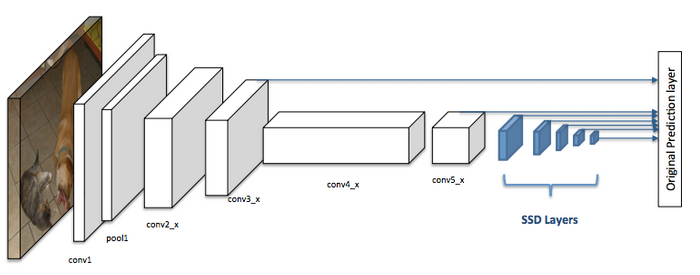
\includegraphics[width=10cm]{imagenes/cnnssd.png}
	\caption{Arquitectura de una CNN con uso de SSD \cite{ssdwork}.}
	\label{fig:ssd}
\end{figure}

Otras característica destacables de SSD es la división de la imagen de entrada mediante un \textit{grid} y realizar una predicción de la clase y la localización del objeto en cada una de las celdas de dicho grid. Si en dicho grid no existe ningún objeto, se considera como \textit{background} y la localización es ignorado. A cada celda se le puede asignar varias \textit{anchor boxes} (\textit{Bounding boxes} con una altura y anchura predefinida) con un tamaño igual al de las celdas. Pero no todos los objetos que están contenidos en la imagen tienen dicho tamaño, por eso se añade un parámetro (\textit{ratio}) dedicado a especificar los diferentes valores que pueden tomar las \textit{anchor boxes}. Asimismo, existe otro parámetro llamado zoom para especificar cuanto pueden escalar dichos \textit{boxes}, tanto aumentando como reduciendo \cite{ssdwork}.

El comportamiento y aportaciones específicas de este modelo, vienen planteadas en el paper con su mismo nombre, \textit{"SSD: Single Shot MultiBox Detector"} \cite{ssd}. Y son las siguientes:

\begin{enumerate}
	\item Se introduce un modelo para la detección de múltiples categorías que es más eficaz y preciso que los modelos posteriores como \textit{YOLO}.
	\item El núcleo de SSD predice la categoría y localización de la \textit{bounding box} mediante el uso de pequeños filtros convolucionales aplicados sobre mapas de características.
	\item Para obtener una mayor precisión se realizan predicciones sobre mapas de características con diferente escalado.
	\item Experimentación con análisis de tiempo y precisión sobre el modelo evaluado sobre \textit{PASCAL VOC}, \textit{COCO} y \textit{ILSVRC}. Asimismo, es comparado con modelos recientes.
\end{enumerate}

MobileNet es un modelo con arquitectura \textit{CNN} para la clasificación de imágenes y visión artificial en móviles. Lo que hace especial este modelo es la potencia computacional necesaria para ejecutarlo o aplicar transfer learning sobre el. Esto lo convierte en un perfecto candidato para dispositivos móviles, sistemas integrados y ordenadores sin GPU o baja eficiencia computacional sin llegar a comprometer significativamente la precisión de los resultados.

Este modelo se basa en el uso de una arquitectura optimizada que utiliza convoluciones separables en profundidad para construir \textit{deep neural networks} ligeros. Además, proporciona dos hiperparámetros globales que permiten ajustar de forma eficiente entre la latencia y precisión. Por consiguiente, con la combinación de ambos, se logra la creación de un modelo apto para dispositivos y ordenadores con poca potencia de GPU, capaz de obtener una detección de forma precisa y veloz.

\newpage
\subsection*{Prototipo}

\vspace{-0.5cm}
\subsubsection*{1. Instalación del framework}
\vspace{-0.7cm}
Para realizar este prototipo se hace uso del API \textit{object\_detection} proporcionado por Tensorflow para Python. Tras seguir las instrucciones ofrecidas se consigue un entorno de trabajo con las siguientes herramientas: Anaconda conjunto a una versión de Python 3.7, Tensorflow, CUDA, TensorFlow Model Garden,  Object Detection API, Protobuf y COCO API.

\vspace{-0.5cm}
\subsubsection*{2. Elección del modelo}
\vspace{-0.7cm}
A la hora de elegir un modelo se tienen en cuenta dos parámetros principales. El primero, Coco mAP (\textit{main Average Prestion}), indica la precisión media del modelo. Mientras que, el segundo, Speed, mide la velocidad de refresco.

\textit{SSD-MobileNetV2} (320x320) será el modelo elegido, ya que dispone de las mejores medidas en cuanto a velocidad. Exactamente cuenta con una medida \textit{Coco mAP} de 20.2 y 19 ms de \textit{Speed}. Aunque la precisión sea más baja que el resto de modelos, se suple con la gran velocidad que logra este modelo.

\vspace{-0.5cm}
\subsubsection*{3. Dataset de imágenes y labeling}
\vspace{-0.7cm}
Para el dataset, se ha realizado una combinación de datasets donde aparecen imágenes de personas con mascarilla, sin ella y con ella pero mal puesta \cite{Cabani_2021} \cite{datasetMask}. Consta de un total de 895 imágenes, dividas en dos grupos train y test. En el primero se encuentran las imágenes que se utilizarán para el entrenamiento del modelo por \textit{Transfer Learning} y cuenta con 745 imágenes. Mientras que, el conjunto de test se utilizará para validar el modelo entrenado con un total de 150 imágenes.

Antes de realizar el modelo es necesario preparar las imágenes conjuntamente a un archivo donde se plasmen las etiquetas del mismo. Para ello, se hace uso de un programa (hecho en Python) llamado \textit{labelImg}. Al tratar las imágenes, se crean unos archivos \textit{xml} donde se encuentra la información del etiquetado que se ha realizado, en este caso se tiene uno de los dos labels del trabajo: \textit{mask} o \textit{noMask}. Una vez creados todos los archivos de etiquetado \textit{xml} con los labels, se tiene que crear un archivo \textit{pbtxt} donde se refleje todas las labels posibles que tendrá el modelo.

En resumen, un \textit{LabelMap} es una archivo referido a enumerar todas las clases posibles en la identificación de objetos. Además, cada una de las imágenes de entrenamiento dispondrá de un archivo adicional donde aparezcan cada \textit{label} de la misma y su localización. Depende del modelo usado, los archivos de \textit{LabelMap} serán de un tipo u otro. En el caso de Tensorflow se utiliza un \textit{TFRecord}, mientras que en YOLO se usa un \textit{txt}.

Por último, se usa un script proporcionado por Tensorflow para transformar el etiquetado que hemos realizado al formato correcto para el entrenamiento del modelo (\textit{TFRecord}).

\vspace{-0.5cm}
\subsubsection*{4. Transfer Learning}
\vspace{-0.7cm}
Antes de hacer el entrenamiento se tiene que preparar un archivo de configuración sobre el modelo seleccionado (SSD-MobileNetV2). Este archivo tiene el nombre de \textit{pipeline.config} y contiene la información principal del modelo, tanto el número de clases que puede detectar, el tamaño que reajusta las imágenes antes de tratarlas y checkpoints para el entrenamiento. Para su creación será necesario el uso de las siguientes herramientas: Tensorflow, Object Detection API y Protobuf. Este último, es una herramienta de Google centrada en transformar los \textit{xml} de etiquetado que hemos creado antes en \textit{protocol buffers}, para poder serializar la información de forma estructurada y más rápida.

Para realizar el entrenamiento se hace uso del código proporcionado tras la instalación de la API Object Detection de Tensorflow, llamado \textit{model\_main\_tf2}. A este hay que cederle la siguiente información: dirección de salida, archivo de configuración y número de pasos de entrenamiento. Tras el entrenamiento, se obtienen unos archivos llamados \textit{checkpoints} con los que se podrá cargar el modelo para su uso mediante la siguientes clases de Tensorflow: \textit{Model\_builder} y \textit{Checkpoint}.

\vspace{-0.5cm}
\subsubsection*{5. Realizar detección}
\vspace{-0.7cm}
Para la detección de la mascarilla se crea una función, \textit{detect\_fn}, que tomando una imagen se pre-procesa con el objetivo de  reducir su tamaño al de la entrada del modelo, siendo en este caso 320x320. Tras esto, se realiza la detección usando el modelo que hemos creado y se realiza un post-procesado para obtener una imagen de salida del mismo tamaño que la de entrada.

El último paso será realizar esta detección en tiempo real, mediante el uso de OpenCV. Una vez capturado un \textit{frame} de la cámara de entrada, se debe transformar en una entrada compatible con el modelo, en este caso un tensor. Con este ya se puede detectar el objeto con la función que se ha definido anteriormente, \textit{detect\_fn}. 

De manera que, cuando se obtiene el label que se ha detectado, se utiliza la herramienta de visualización de la API Object Detection, \textit{visualization\_utils}, para mostrar el resultado por pantalla. Un ejemplo del funcionamiento se puede observar en la \textit{Figura \ref{fig:protoTensorFlow}}.

\begin{figure}[htp]
	\centering
	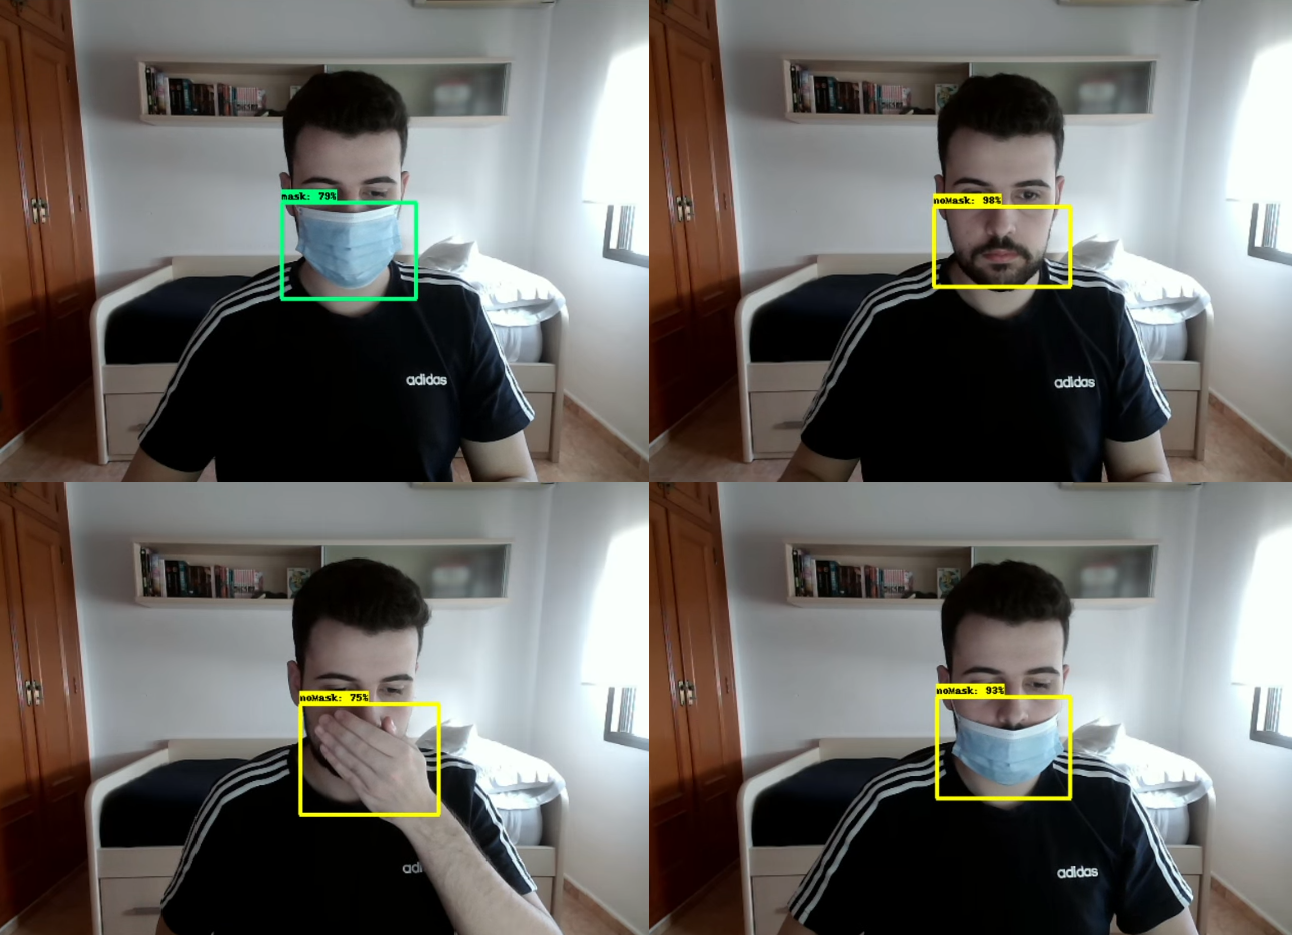
\includegraphics[width=12cm]{imagenes/tf_prueba.png}
	\caption{Pruebas con SSD-MobileNetV2.}
	\label{fig:protoTensorFlow}
\end{figure}

El tiempo de retardo que presenta este prototipo para el PC1 es de una media de 83.2 ms. El resultado obtenido sea bastante bueno, cuando solamente funciona en un ámbito cerrado. Esto se debe a que el entrenamiento del modelo usado se ha realizado con imágenes mías. Aun así, este prototipo tras un entrenamiento con un dataset más amplio, funciona de forma correcta pero con más errores. Destacando que su funcionamiento correcto sucede en una distancia a cámara muy cercana. Cuanto más lejos se sitúe la persona de la cámara, más detecciones falsas se crearán, sobre todo en el caso de encontrar una mascarilla cuando no la hay. Este puede mejorar su funcionamiento si se realiza un dataset más amplio aún y un entrenamiento más largo. De igual forma, si se encuentra en una situación donde la iluminación sea escasa o la cámara no este bien colocada el rendimiento del prototipo disminuye.

\newpage
\section{Comparación}

Este apartado estará dedicado a la comparación de los prototipos implementados anteriormente, con el objetivo de contrastar el funcionamiento de todos ellos y las técnicas implementadas. Para ello, se hará uso de dos medidas: distancia de funcionamiento y el tiempo que tarda en procesar una imagen.

\subsection*{Distancia}
\vspace{-0.5cm}
La primera comparación se basa en el estudio del rango de funcionamiento de los prototipos. Pudiendo medir su distancia mediante el tamaño de la imagen que se le pasa como entrada al algoritmo. En la siguiente tabla (Cuadro \ref{tab:table3}) se presenta esto mediante una medida en píxeles (x,y) que corresponde con la medida de la detección más pequeña que el prototipo puede procesar. Además, aparecerán dos medidas: la primera cuando no se lleva mascarilla y la segunda cuando si.

\begin{table}[h!]
	\begin{center}
		\begin{tabular}{ |c|c|c|c| } 
			\hline
			\textbf{Prototipo 1} & \textbf{Prototipo 2} & \textbf{Prototipo 3} & \textbf{Prototipo 4} \\
			\hline
			(25,25) & (32,32)  & (18,26) & (320, 320)* \\
			(25,25) & (68,68)  & (38,44) & (320, 320)* \\
			\hline
		\end{tabular}
		\caption{Rango píxeles de los prototipos.}
		\label{tab:table3}
	\end{center}
\end{table}

En el caso del último prototipo todas las imágenes que procesa son re-escaladas a unas dimensiones de 320x320, debido a las características que presenta el mismo. Obteniendo como resultado, detecciones con unos píxeles cercanos a estos valores.

En conclusión, como resultado final se obtiene que el prototipo 1, a pesar de no utilizar técnicas avanzadas de \textit{deep learning}, obtiene el mejor resultado de los cuatro prototipos. Pudiendo detectar rostros de hasta 25x25 píxeles dentro de la imagen de entrada.

\vspace{-0.5cm}
\subsection*{Tiempo de retardo}
\vspace{-0.5cm}

La segunda comparación se basa en la medida del tiempo que toma el algoritmo en tratar una imagen de entrada. Para ello se realizará la misma prueba en todos los prototipos, mostrando en la siguiente tabla (Cuadro \ref{tab:table4}) el tiempo medio (ms) tras una ejecución de un minuto.

\begin{table}[h!]
	\begin{center}
		\begin{tabular}{ |c|c|c|c| } 
			\hline
			\textbf{Prototipo 1} & \textbf{Prototipo 2} & \textbf{Prototipo 3} & \textbf{Prototipo 4} \\
			\hline
			87.5 ms & 14.7 ms  & 12.3 ms & 83.2 ms \\
			\hline
		\end{tabular}
		\caption{Tiempo de los prototipos.}
		\label{tab:table4}
	\end{center}
\end{table}

El resultado del estudio presenta al prototipo 3 como el más veloz , mientras que el prototipo 1 como el más lento. Esto se debe a la tecnología implementada en el tercer prototipo, que presenta un modelo \textit{deep learning} centrado en realizar un trabajo rápido en cualquier dispositivo, incluyendo móviles.

De ello resulta necesario decir, que no hay ningún prototipo capaz de destacar en todos los ámbitos, haciendo imposible la selección de una solución general para el problema. Todas las técnicas usadas en este trabajo son capaces de resolverlo, y dependiendo de donde se tenga que implementar el prototipo se tendría que realizar otro estudio para resolver los objetivos del cliente. Por ejemplo,  si se desea implementar un detector de este tipo en un dispositivo móvil o en un sistema embebido, se buscaría un prototipo que sea rápido y poco pesado, como el tercer prototipo (Mediapipe). Mientras que, si se dispone de un dispositivo con más potencia de computo se podría plantear usar un prototipo más lento pero preciso como el primer prototipo (Haar-like features) o incluso entrenar un modelo personalizado como el cuarto prototipo (Transfer Learning). Aun así, se debería de realizar un estudio previo en el dispositivo donde se implementará el prototipo para poder realizar una decisión definitiva.  




% Conclusiones y vias futuras
%!TEX root = proyecto.tex

\chapter{Conclusiones y vías futuras}

Durante el desarrollo de este trabajo se han estudiado y probado la utilización de cuatro técnicas sobre la tarea de detección facial con mascarilla, para asegurar el cumplimiento de las normas COVID-19 impuestas por la OMS (Organización Mundial de la Salud). Estas técnicas son las siguientes: Haa-like feature, Facial Landmarks, Mediapipe y Transfer Learning.

Según los resultados obtenidos durante el estudio se concluye en que las técnicas presentadas consiguen realizar detecciones de rostros con mascarillas, cumpliendo así el primer objetivo impuesto. Los mejores resultados se logran con el primer prototipo, centrado en el uso de \textit{Haar-like features} combinado con \textit{Machine Learning} para la creación de un modelo apto para medir el cumplimiento de las normas COVID-19, durante una ejecución en tiempo real. Mientras que, el cuarto prototipo es el que mejor resultado bajo las pruebas realizadas con el dataset. De igual forma, el resto de técnicas son capaces de realizar dicha tarea, destacando el buen rendimiento del prototipo con Mediapipe y los malos resultados de \textit{Facial Landmark}, incapaz de detectar el rostro con mascarilla en muchas ocasiones.

De forma análoga, un prototipo de los desarrollados es capaz de reconocer cuando la persona detectada viste mal la mascarilla, siendo el caso de Transfer Learning y Tensorflow. Gracias a la creación de un modelo adaptado a estas necesidades, pero unicamente logrando un buen funcionamiento en situaciones ideales: buena luz y cercanía a la cámara. Finalmente, es importante destacar el último de los objetivos: tratar los falsos positivos. Los prototipos creados a partir de Haar-like feature, Facial Landmarks y Mediapipe presentan dicha característica, ya que realizan detecciones de 'llevar mascarillas' en situaciones donde la persona no la lleva, por ejemplo: cuando la persona obstaculiza la visibilidad de la boca. El motivo proviene de la naturaleza de estos prototipos, dado que basan su funcionamiento en el uso del reconocimiento de características, y al no encontrar la boca se detecta el uso de mascarilla. El único caso apto para este objetivo es el prototipo de Tensorflow, comentado anteriormente.

A lo largo del desarrollo de este trabajo se ha aprendido a emplear herramientas como Python, Tensorflow, frameworks de Python (Mediapipe, Dlib, Numpy) y OpenCV. Además, de profundizar en términos e ideas del \textit{Machine Learning}, visión artificial y \textit{Deep Learning}.

A modo de cierre, se pueden desatacar las siguientes vías futuras para continuar este trabajo:
\begin{itemize}
	\item Realizar más pruebas en distintos dispositivos (ordenadores, móviles, sistemas embebidos).
	\item Ampliar el funcionamiento de los prototipos. Creando modelos más completos.
	\item Utilizar servicios en la nube para implementar los prototipos.
	\item Realizar el estudio de más técnicas.
	\item Añadir más normas COVID-19 en los prototipos.
\end{itemize}

% Apéndices, si hiciese falta
%\appendix
%%!TEX root = proyecto.tex

\chapter{ANEXO I - Implementación Viola-Jones Face Detector}
%%!TEX root = proyecto.tex

\chapter{ANEXO II - Implementación Dlib Facial Landmarks}



\nocite{*}

\begin{spacing}{1}
	\bibliography{bibliografia}
	\addcontentsline{toc}{chapter}{Bibliografía}
	\bibliographystyle{plainurl}
\end{spacing}


\end{document}
